\documentclass{csse4400}

\usepackage{languages}

\title{Getting Started with the Cloud}
\author{Brae Webb \& Richard Thomas}

\date{\week[practical]{4}}
\begin{document}

\maketitle

\begin{figure}[h]
  \begin{center}
    
\includegraphics[scale=0.4]{images/hextriscloud}
  \end{center}
\end{figure}

% \section{Before Class}
% It's preferable if you already have \link{terraform installed}{https://learn.hashicorp.com/tutorials/terraform/install-cli}.
% Please also have one of IntelliJ IDEA, PyCharm, or VSCode with the terraform plugin installed.

\section{This Week}
This week our goal is to get acquainted with AWS Academy.
Throughout the course we will use AWS Academy to learn how to deploy and manage infrastructure with AWS.
Additionally, AWS Academy will be used to develop the Cloud assignment.
Specifically, this week you need to:
\begin{itemize}
    \item Enrol in
    \begin{enumerate}
        \item AWS Academy Cloud Foundations [\href{https://awsacademy.instructure.com/courses/73523}{73523}] course;
        \item AWS Academy Learner Lab [\href{https://awsacademy.instructure.com/courses/73527}{73527}] course;
        \item AWS Academy Cloud Architecting [\href{https://awsacademy.instructure.com/courses/73526}{73526}] course; and
        \item AWS Academy Cloud Developing [\href{https://awsacademy.instructure.com/courses/73525}{73525}] course.
    \end{enumerate}
    \item Navigate the AWS Academy interface.
    \item Enter the AWS Console from an AWS Academy lab.
    \item Provision an EC2 instance that deploys a simple static website.
\end{itemize}

We will then start using an Infrastructure as Code tool,
specifically, Terraform,
to deploy the static website instead of using the AWS Console.
Specifically, this week you need to:
\begin{itemize}
    \item Authenticate Terraform to use the AWS learner lab.
    \item Configure a single server website in Terraform and deploy.
    \item Create a Terraform module for deploying arbitrary single server websites.
\end{itemize}

\section{AWS Academy}
AWS Academy is an educational platform to support teaching AWS services.
In this course, we will be using it in two ways:
\begin{enumerate}
    \item The AWS Cloud Foundations, Cloud Architecting, and Cloud Developing courses are supplementary material to help cement your ability to use AWS.
        You are encouraged to work your way through at leas the AWS Cloud Foundations and Cloud Architecting courses.
    \item The AWS Learner Lab provides access to an environment which will be used in these practicals to learn AWS. 
        Later Learn Labs will be used to develop your Cloud Infrastructure assignment.
\end{enumerate}

\section{Enrol in AWS Academy}

\begin{enumerate}
    \item
        Set up your AWS Academy account by responding to your email invitation and clicking \textbf{Get Started}.
        The email invitation will come from AWS Academy.
        Check your junk/spam folders.

        
\includegraphics[width=0.8\textwidth]{images/email-invite}

    \item Go to \url{https://www.awsacademy.com/vforcesite/LMS_Login} to login.
    \begin{enumerate}
        \item Press \textbf{Student Login}.
        \item Use the email address that received the email invitation.
    \end{enumerate}

    \hspace{9mm}
    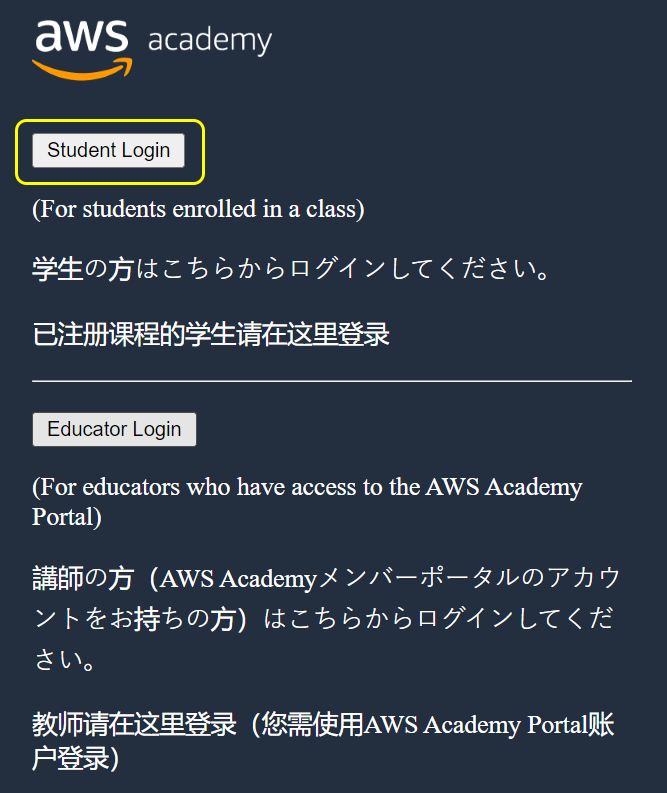
\includegraphics[height=0.35\textheight]{images/labs-login1}
    \hspace{5mm}
    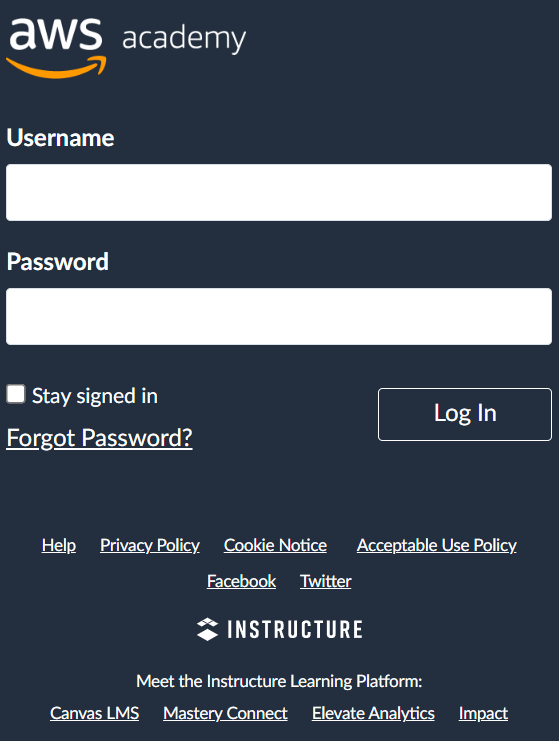
\includegraphics[height=0.35\textheight]{images/labs-login2}
\end{enumerate}


\section{Exploring the Interface}
\aside{We will just be looking at the learner lab today, please ask on the Ed Discussion board if you need help using the supplementary AWS Academy courses.}

Enter the learner lab via the following steps.

\begin{enumerate}

\item Once you have enrolled in the course, you should see the course page.

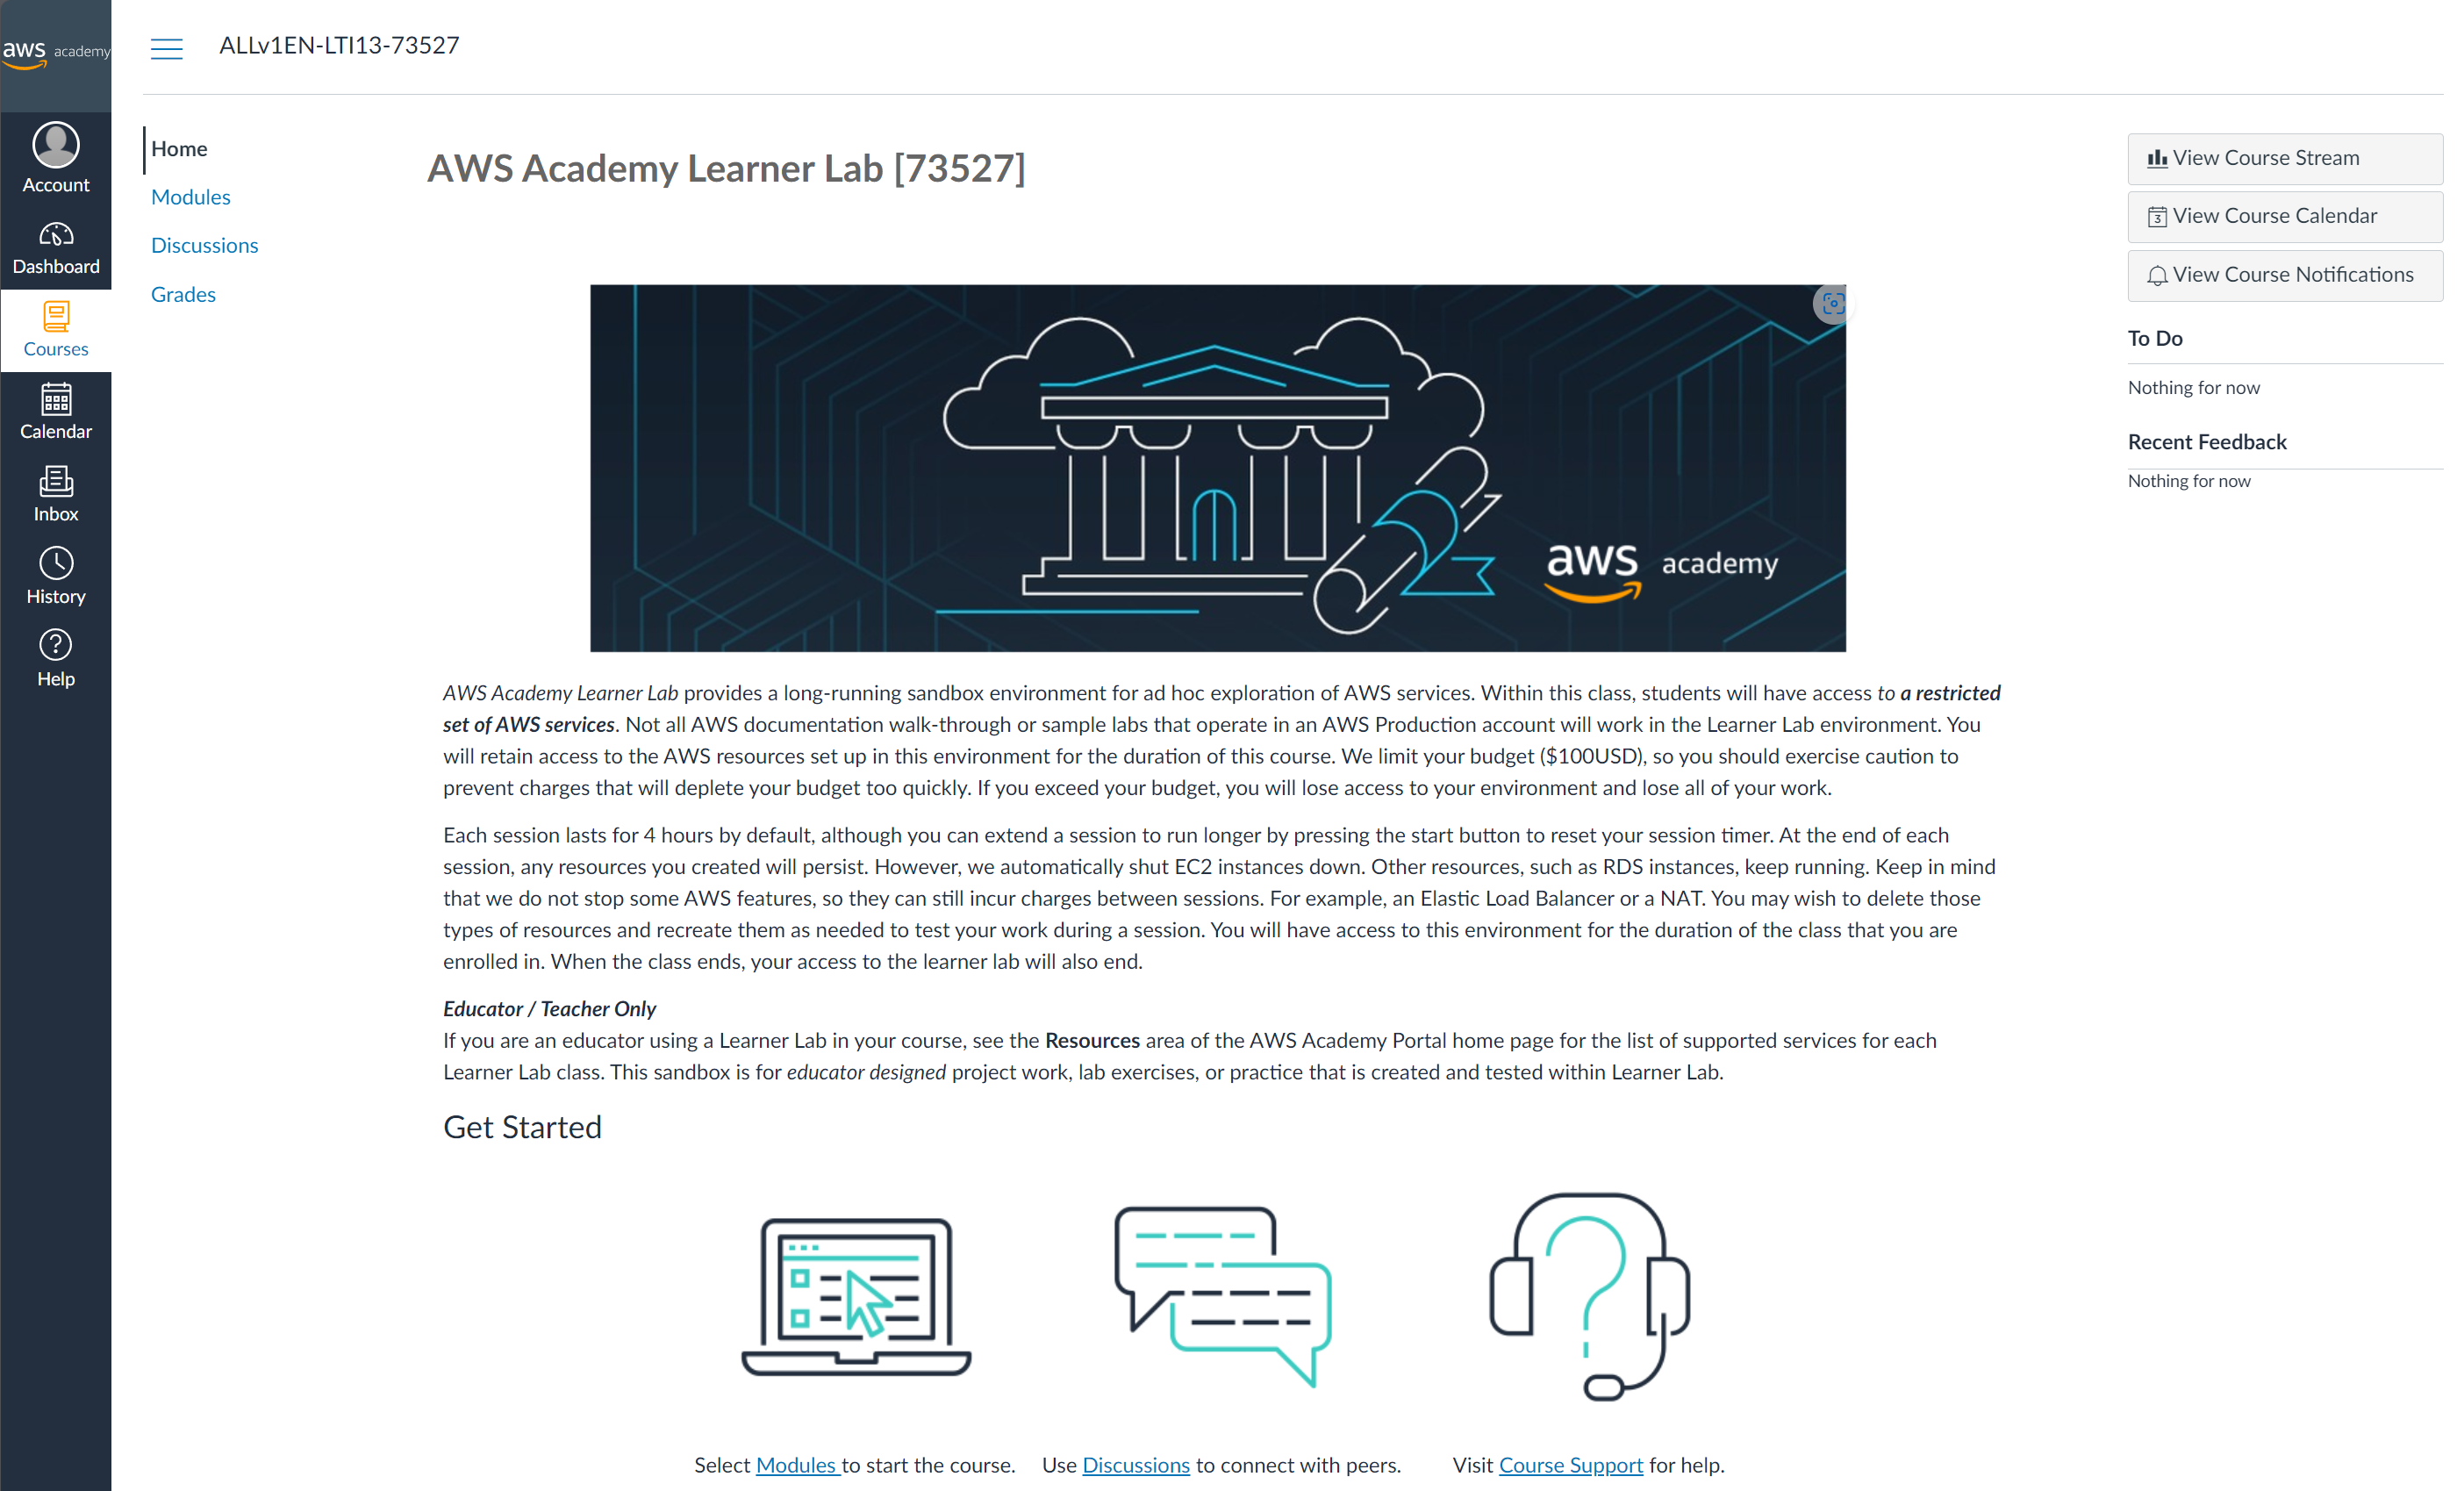
\includegraphics[trim=0 200 0 0,clip,width=0.95\textwidth]{images/academy-homepage}

\item Navigate to the \texttt{Modules} tab and select the link for ``Launch AWS Academy Learner Lab''.
        You will need to accept the AWS Learner Lab terms and conditions to be able to launch learner lab.
        You may also open and browse the ``AWS Academy Learner Lab Student Guide'' and
        ``Learn how to effectively use the AWS Academy Learner Lab'' links which cover some of the content of this practical.

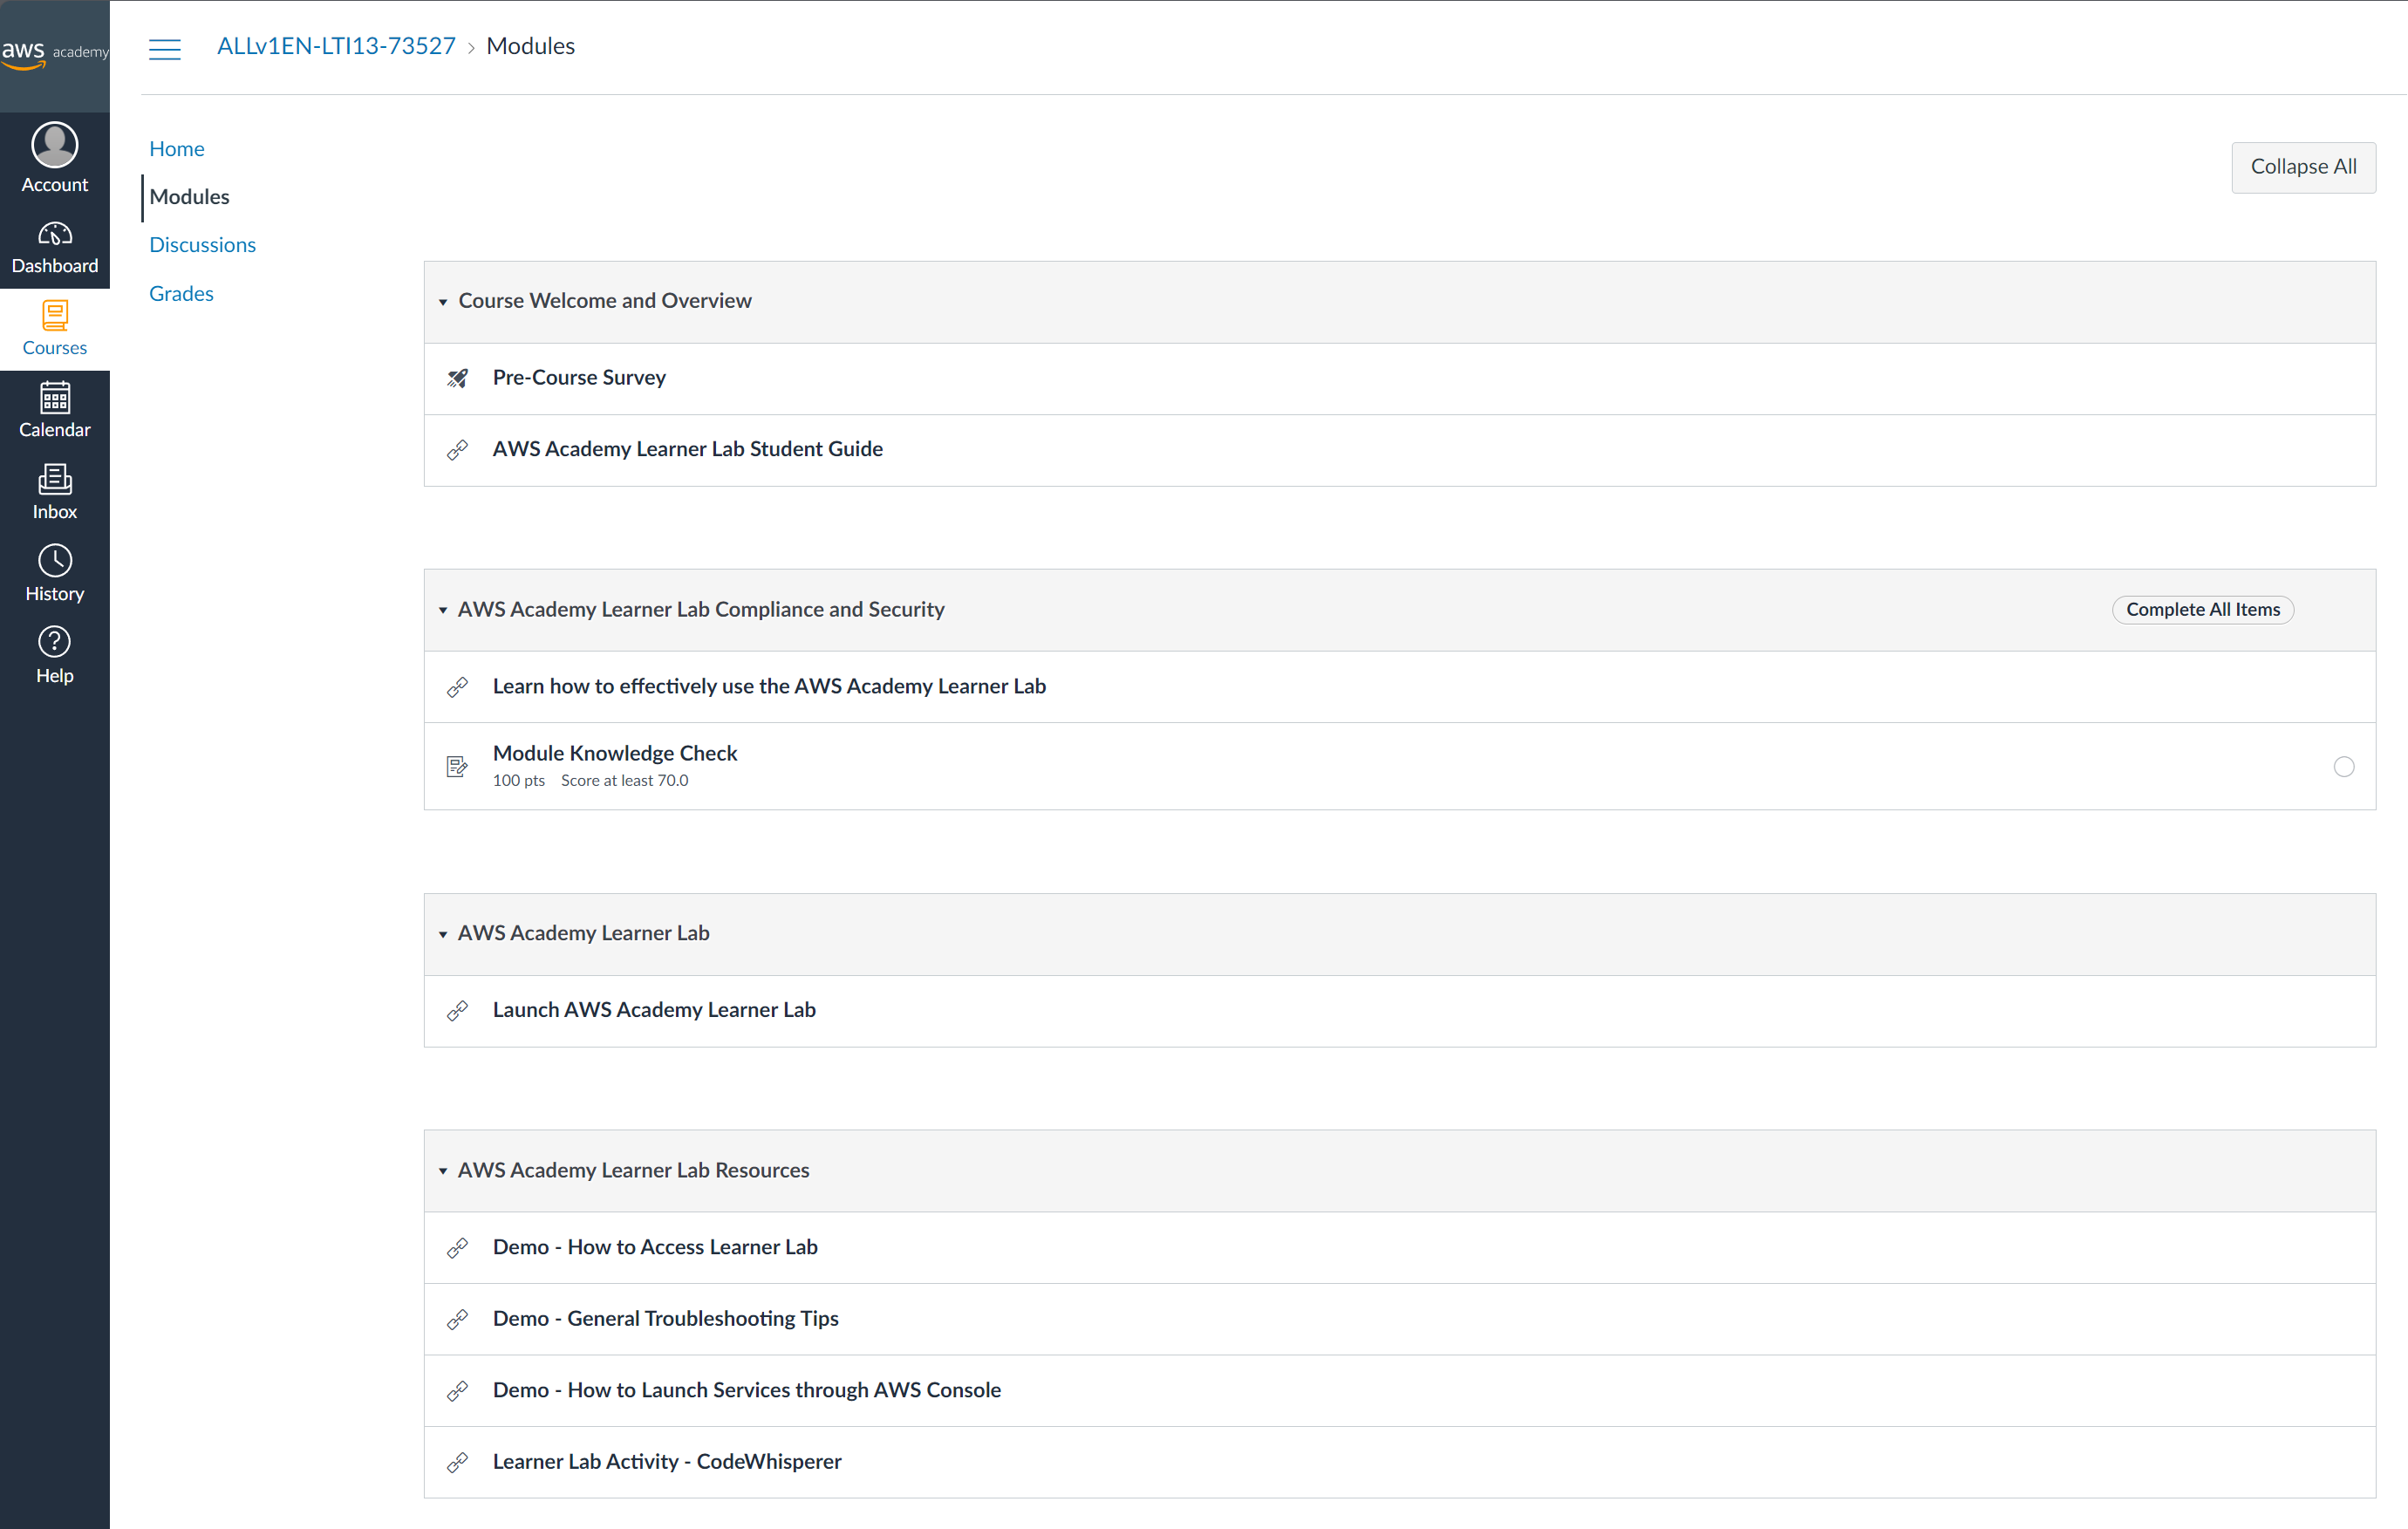
\includegraphics[width=0.95\textwidth]{images/modules-page}

\item You should now see the learner lab interface.
\begin{itemize}
      \item The AWS text, near the top left of the window, with the (currently) red circle is the link to open the AWS console.
      \item You can also see your budget. Note that the budget is not updated in real-time, so avoid creating multiple resources at once.
      \item The \texttt{00:00} is a countdown of hours remaining for your lab.
      A lab can only remain active for 4 hours, after which it will close, unless you press start lab again before the 4 hours expires.
      Once the lab is started, \texttt{00:00} will change to \texttt{04:00}.
      \item AWS details will become important later but are not needed now.
      \item The README button will re-open the text panel currently on the right of the terminal interface.
      \item The README text has a lot of important information including what AWS services are available in the learner labs environment, please read it.
      \item The terminal interface is an environment with the SSH keys required to connect to AWS instances semi-automatically (we will use this today).
\end{itemize}

\hspace{-6mm}
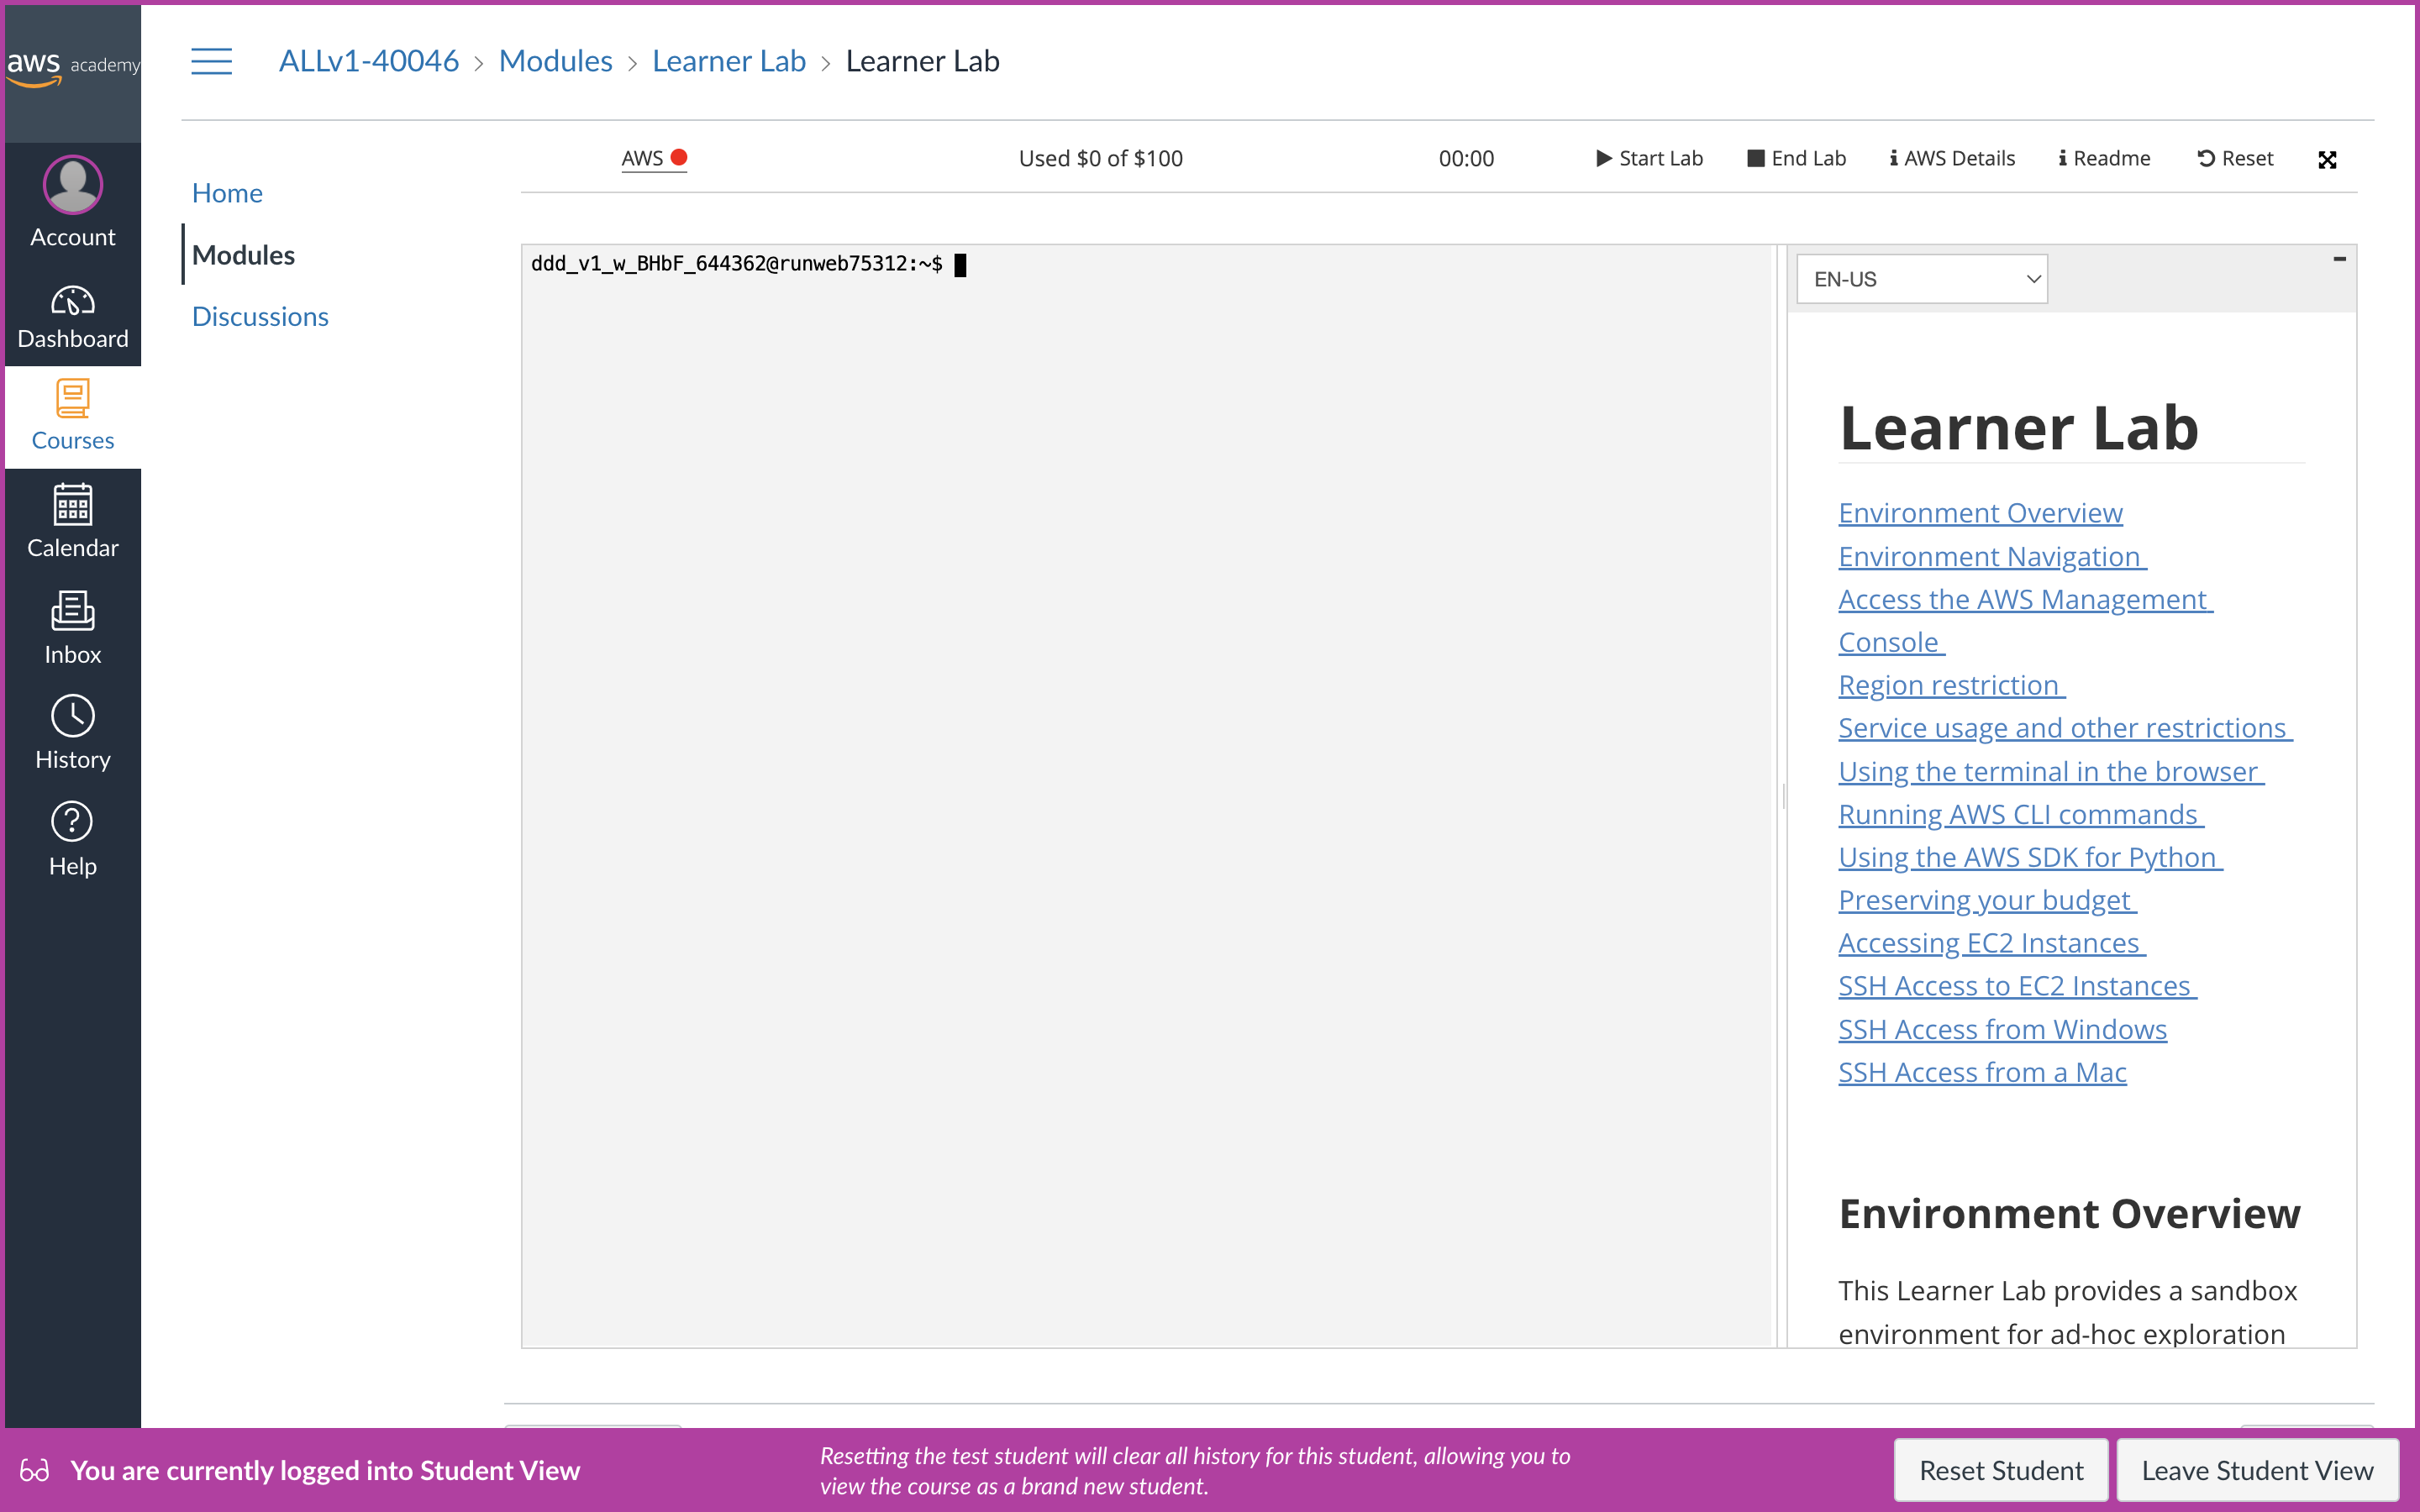
\includegraphics[width=\textwidth]{images/lab-interface}

\item Go ahead and start the lab. It will take a few moments to get ready.
      The red circle will turn yellow as the lab is starting, and green once it has started.
      Click on the green circle when it is available.
      This will open the AWS Console in a new browser tab.
      If you end up working for a company which uses AWS, welcome to your new home.

\teacher{It can take much more than a few moments for some students.}

\hspace{-6mm}
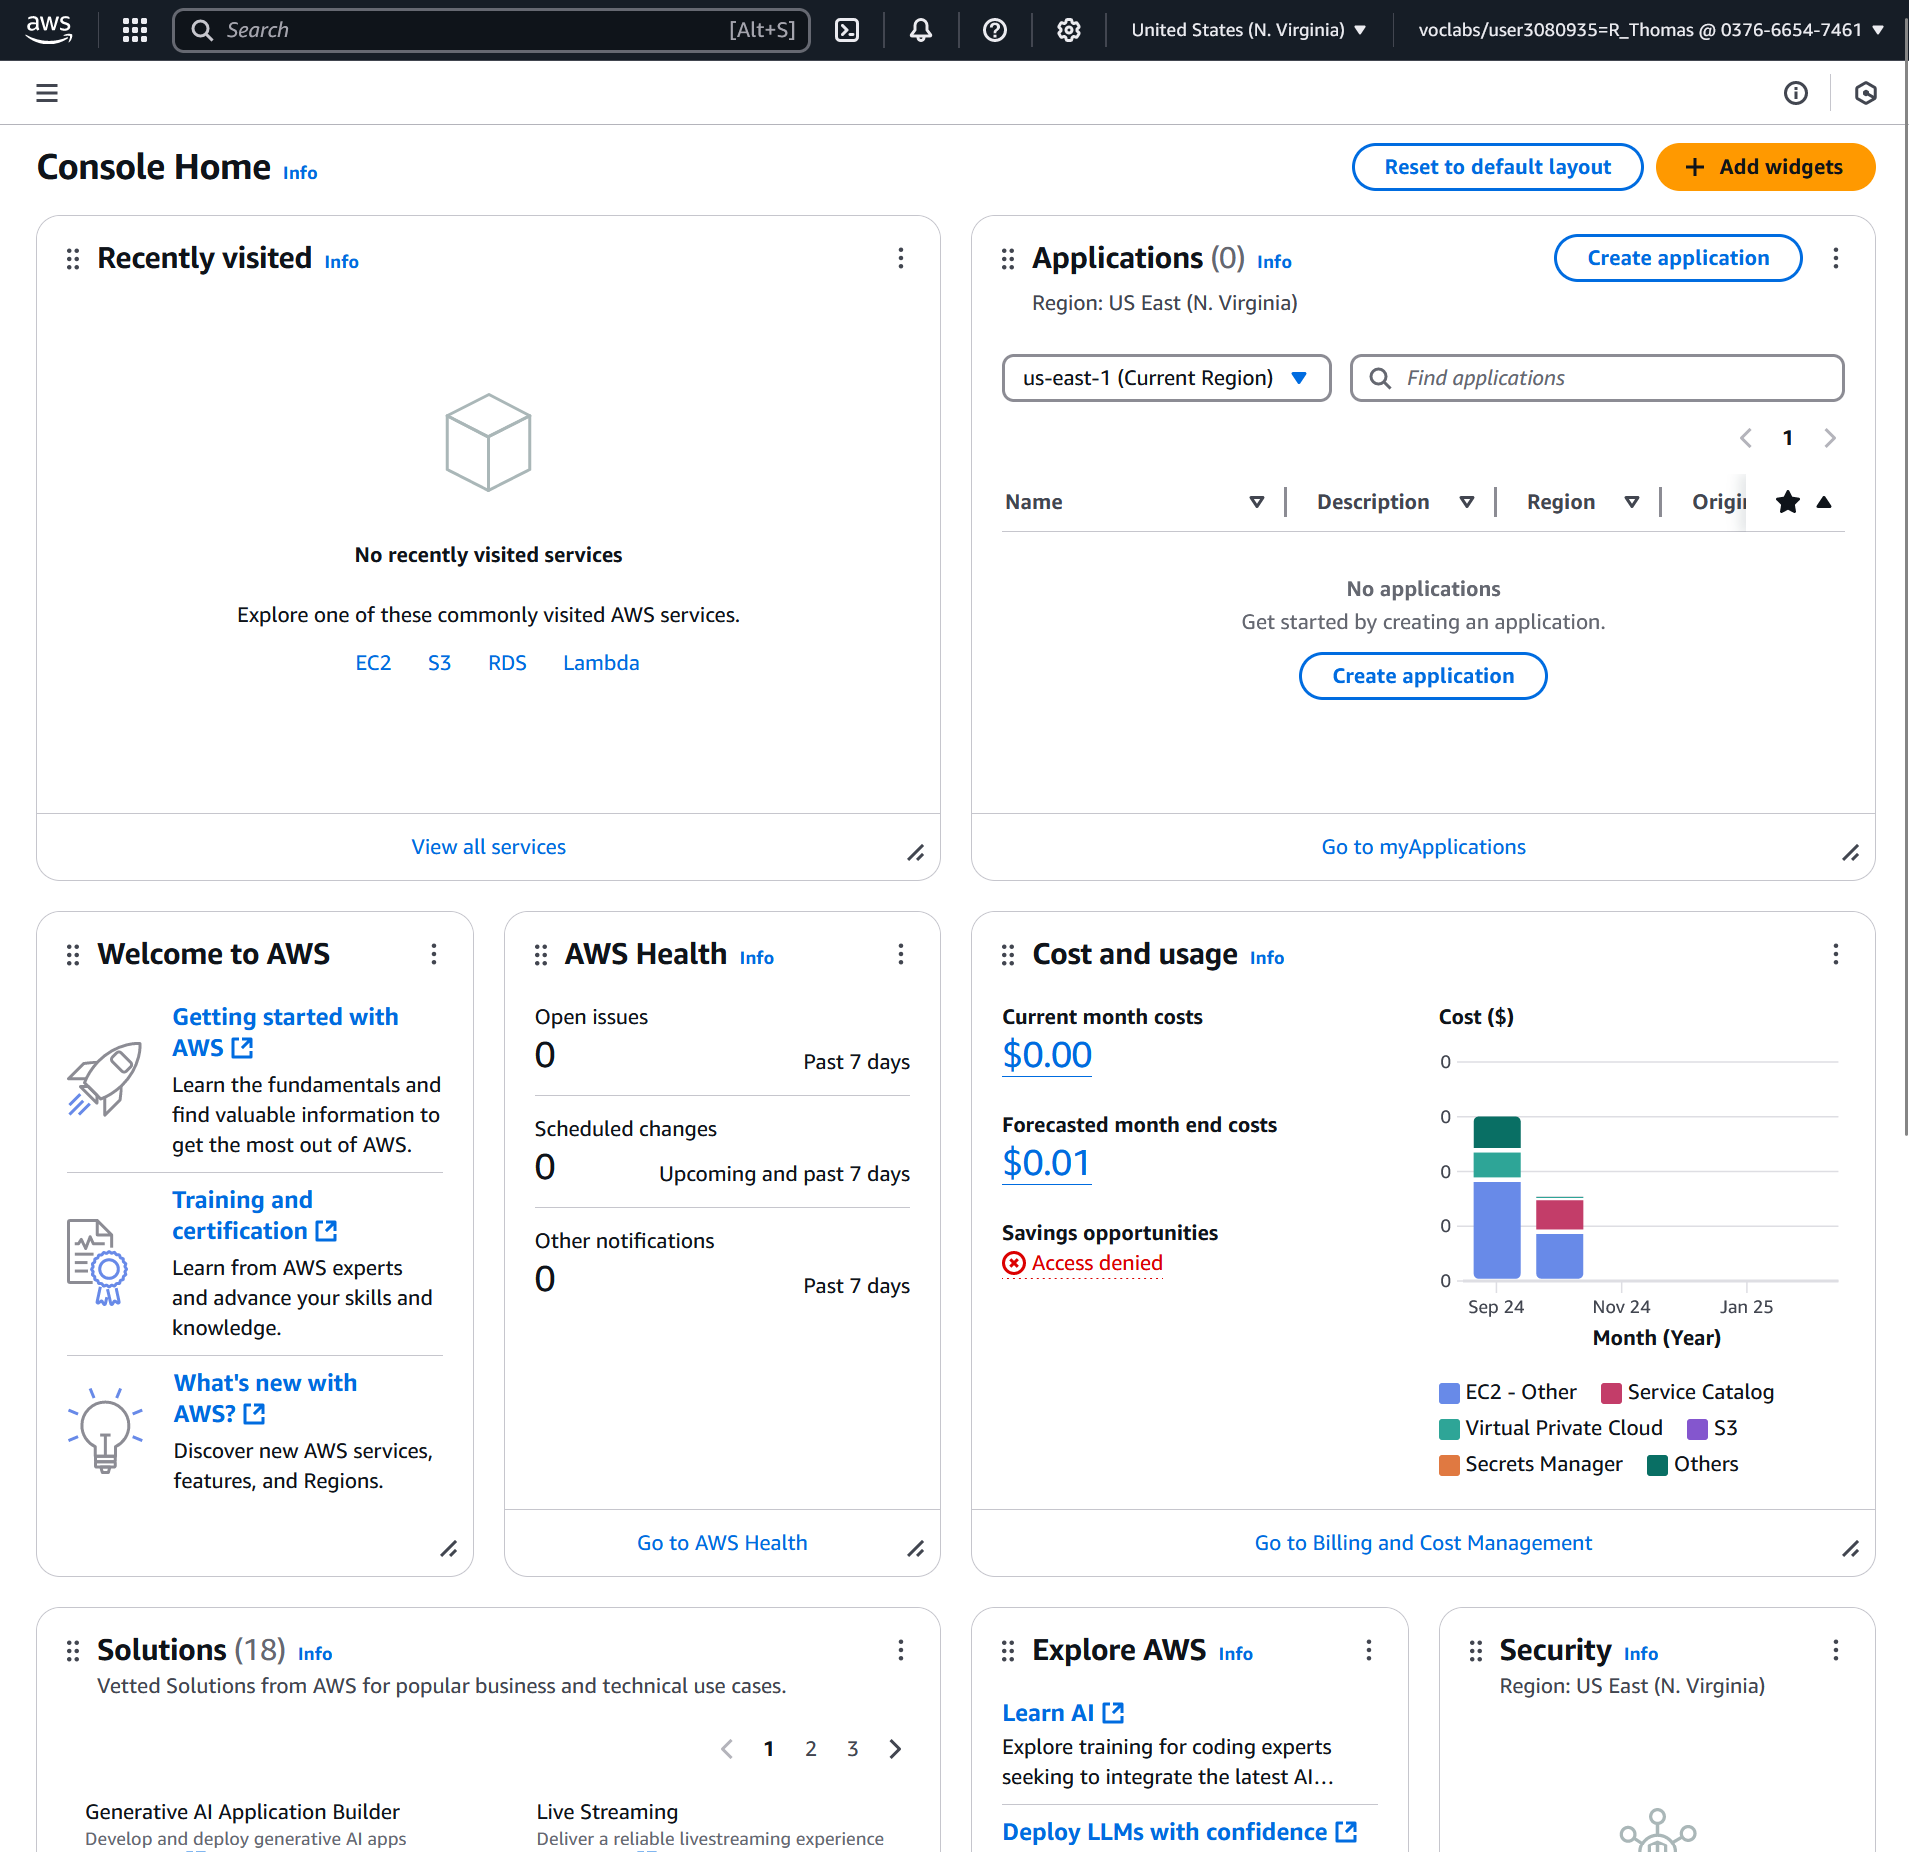
\includegraphics[width=\textwidth]{images/aws-console}

\end{enumerate}

\vspace{3mm}
\aside{Amazon Web Services (AWS) is an
Infrastructure as a Service (IaaS)
and Software as a Service (SaaS) provider.
They offer a collection of services which are helpful for development.
For example, they offer virtual compute resources, database storage options, and networking to tie it all together.
Services are offered on a pay as you go model, meaning you only pay for the seconds you use a service.
We will now get acquainted with some simple services offered by AWS.}

\section{AWS EC2}

Today we are going to focus on using AWS's EC2 service.
Elastic Compute Cloud (EC2) is the primary compute service offered by AWS.
It allows you to create virtual machines on Amazon's infrastructure.
You have full control over this machine and can configure it for whatever purpose you need.

Navigate to the search bar in the top left and find the EC2 service.
You might find this interface overwhelming.
It is important to note that since EC2 is one of the primary services offered by AWS,
many smaller services we do not need are bundled into the service.

\teacher{The foundation course has a module (6) that covers EC2 in more depth, feel free to direct students to it for after the Hextris example.}

\vspace{2mm}
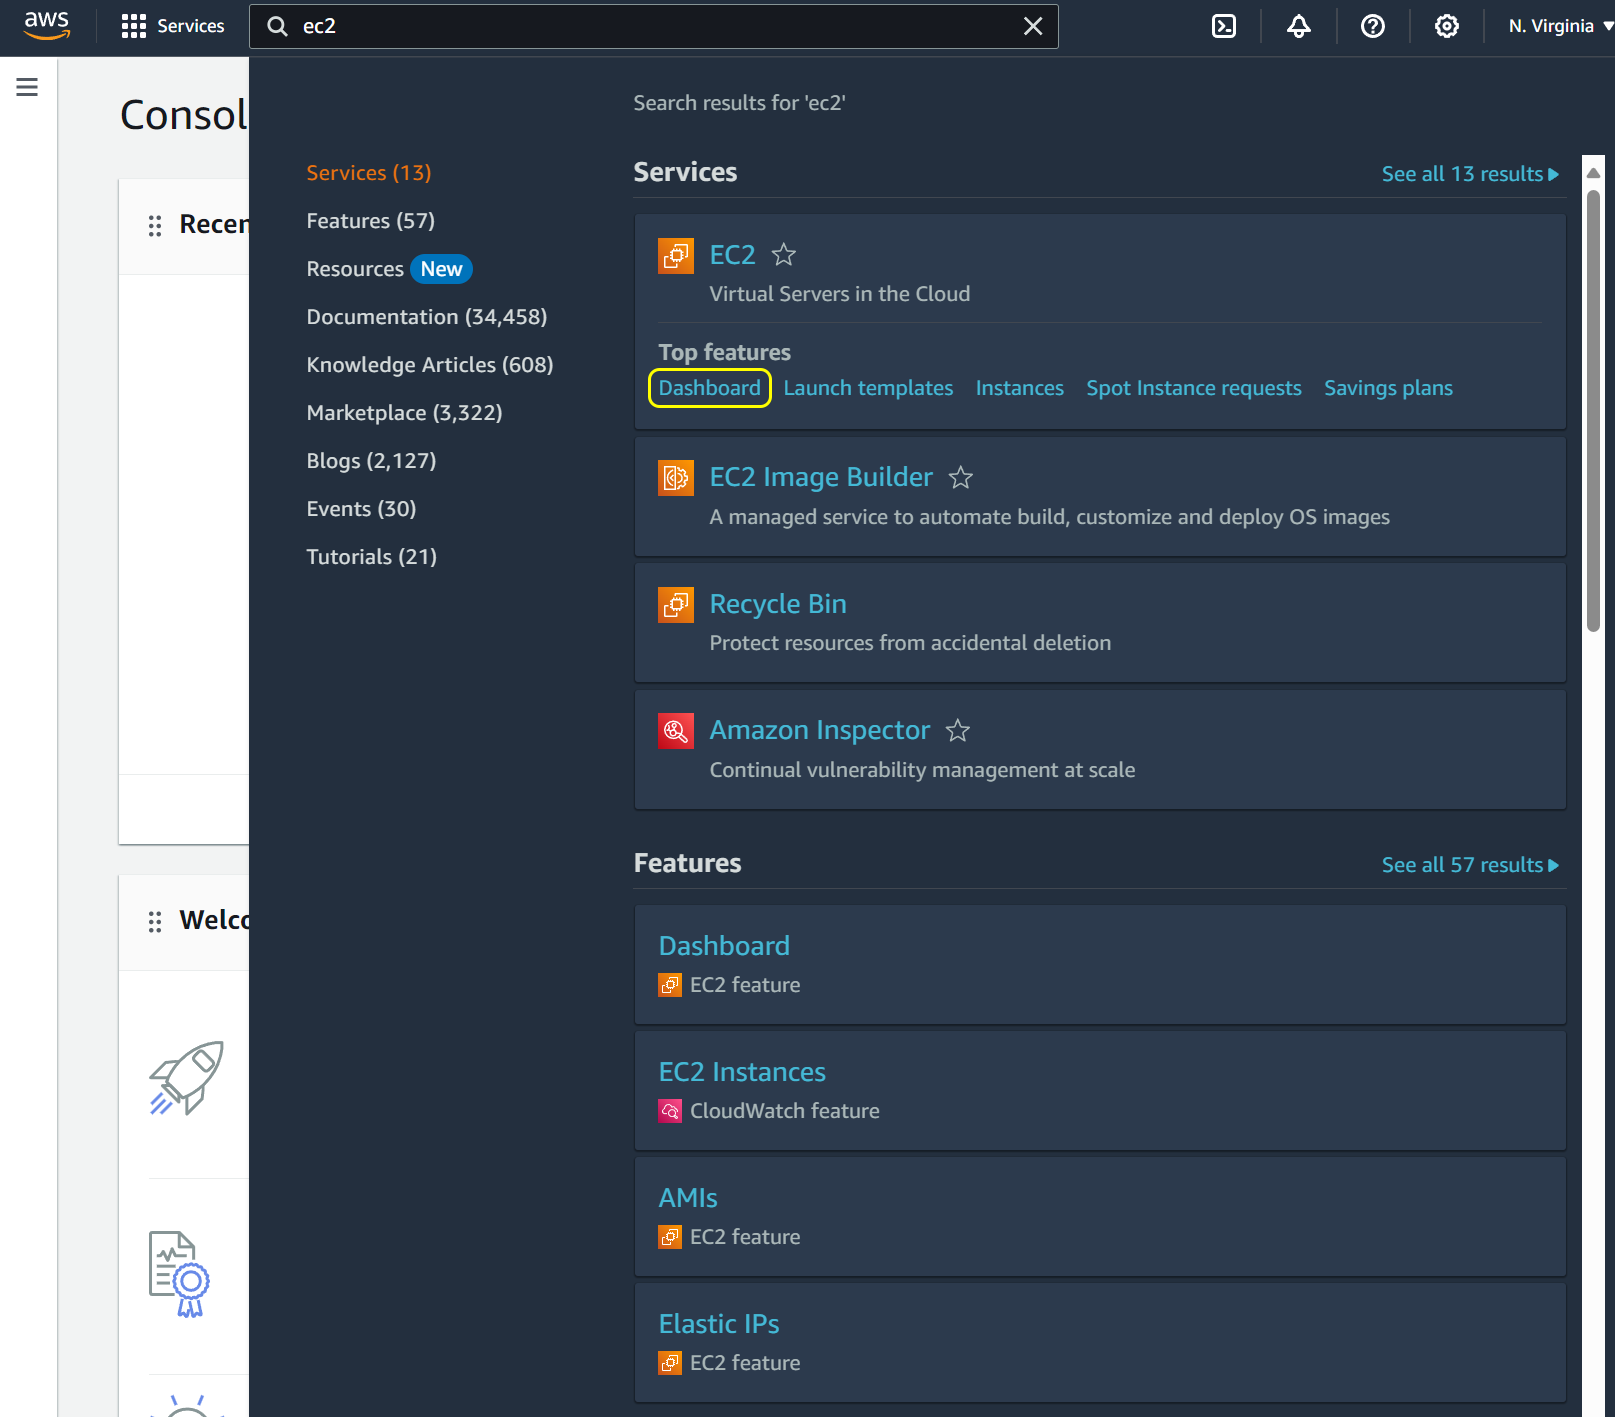
\includegraphics[trim=0 200 0 0,clip,width=0.95\textwidth]{images/search-ec2}
\vspace{5mm}

\noindent
Today, we only need the \texttt{Instances} dashboard.
Navigate to there and select ``Launch instance''.

\vspace{5mm}
\noindent
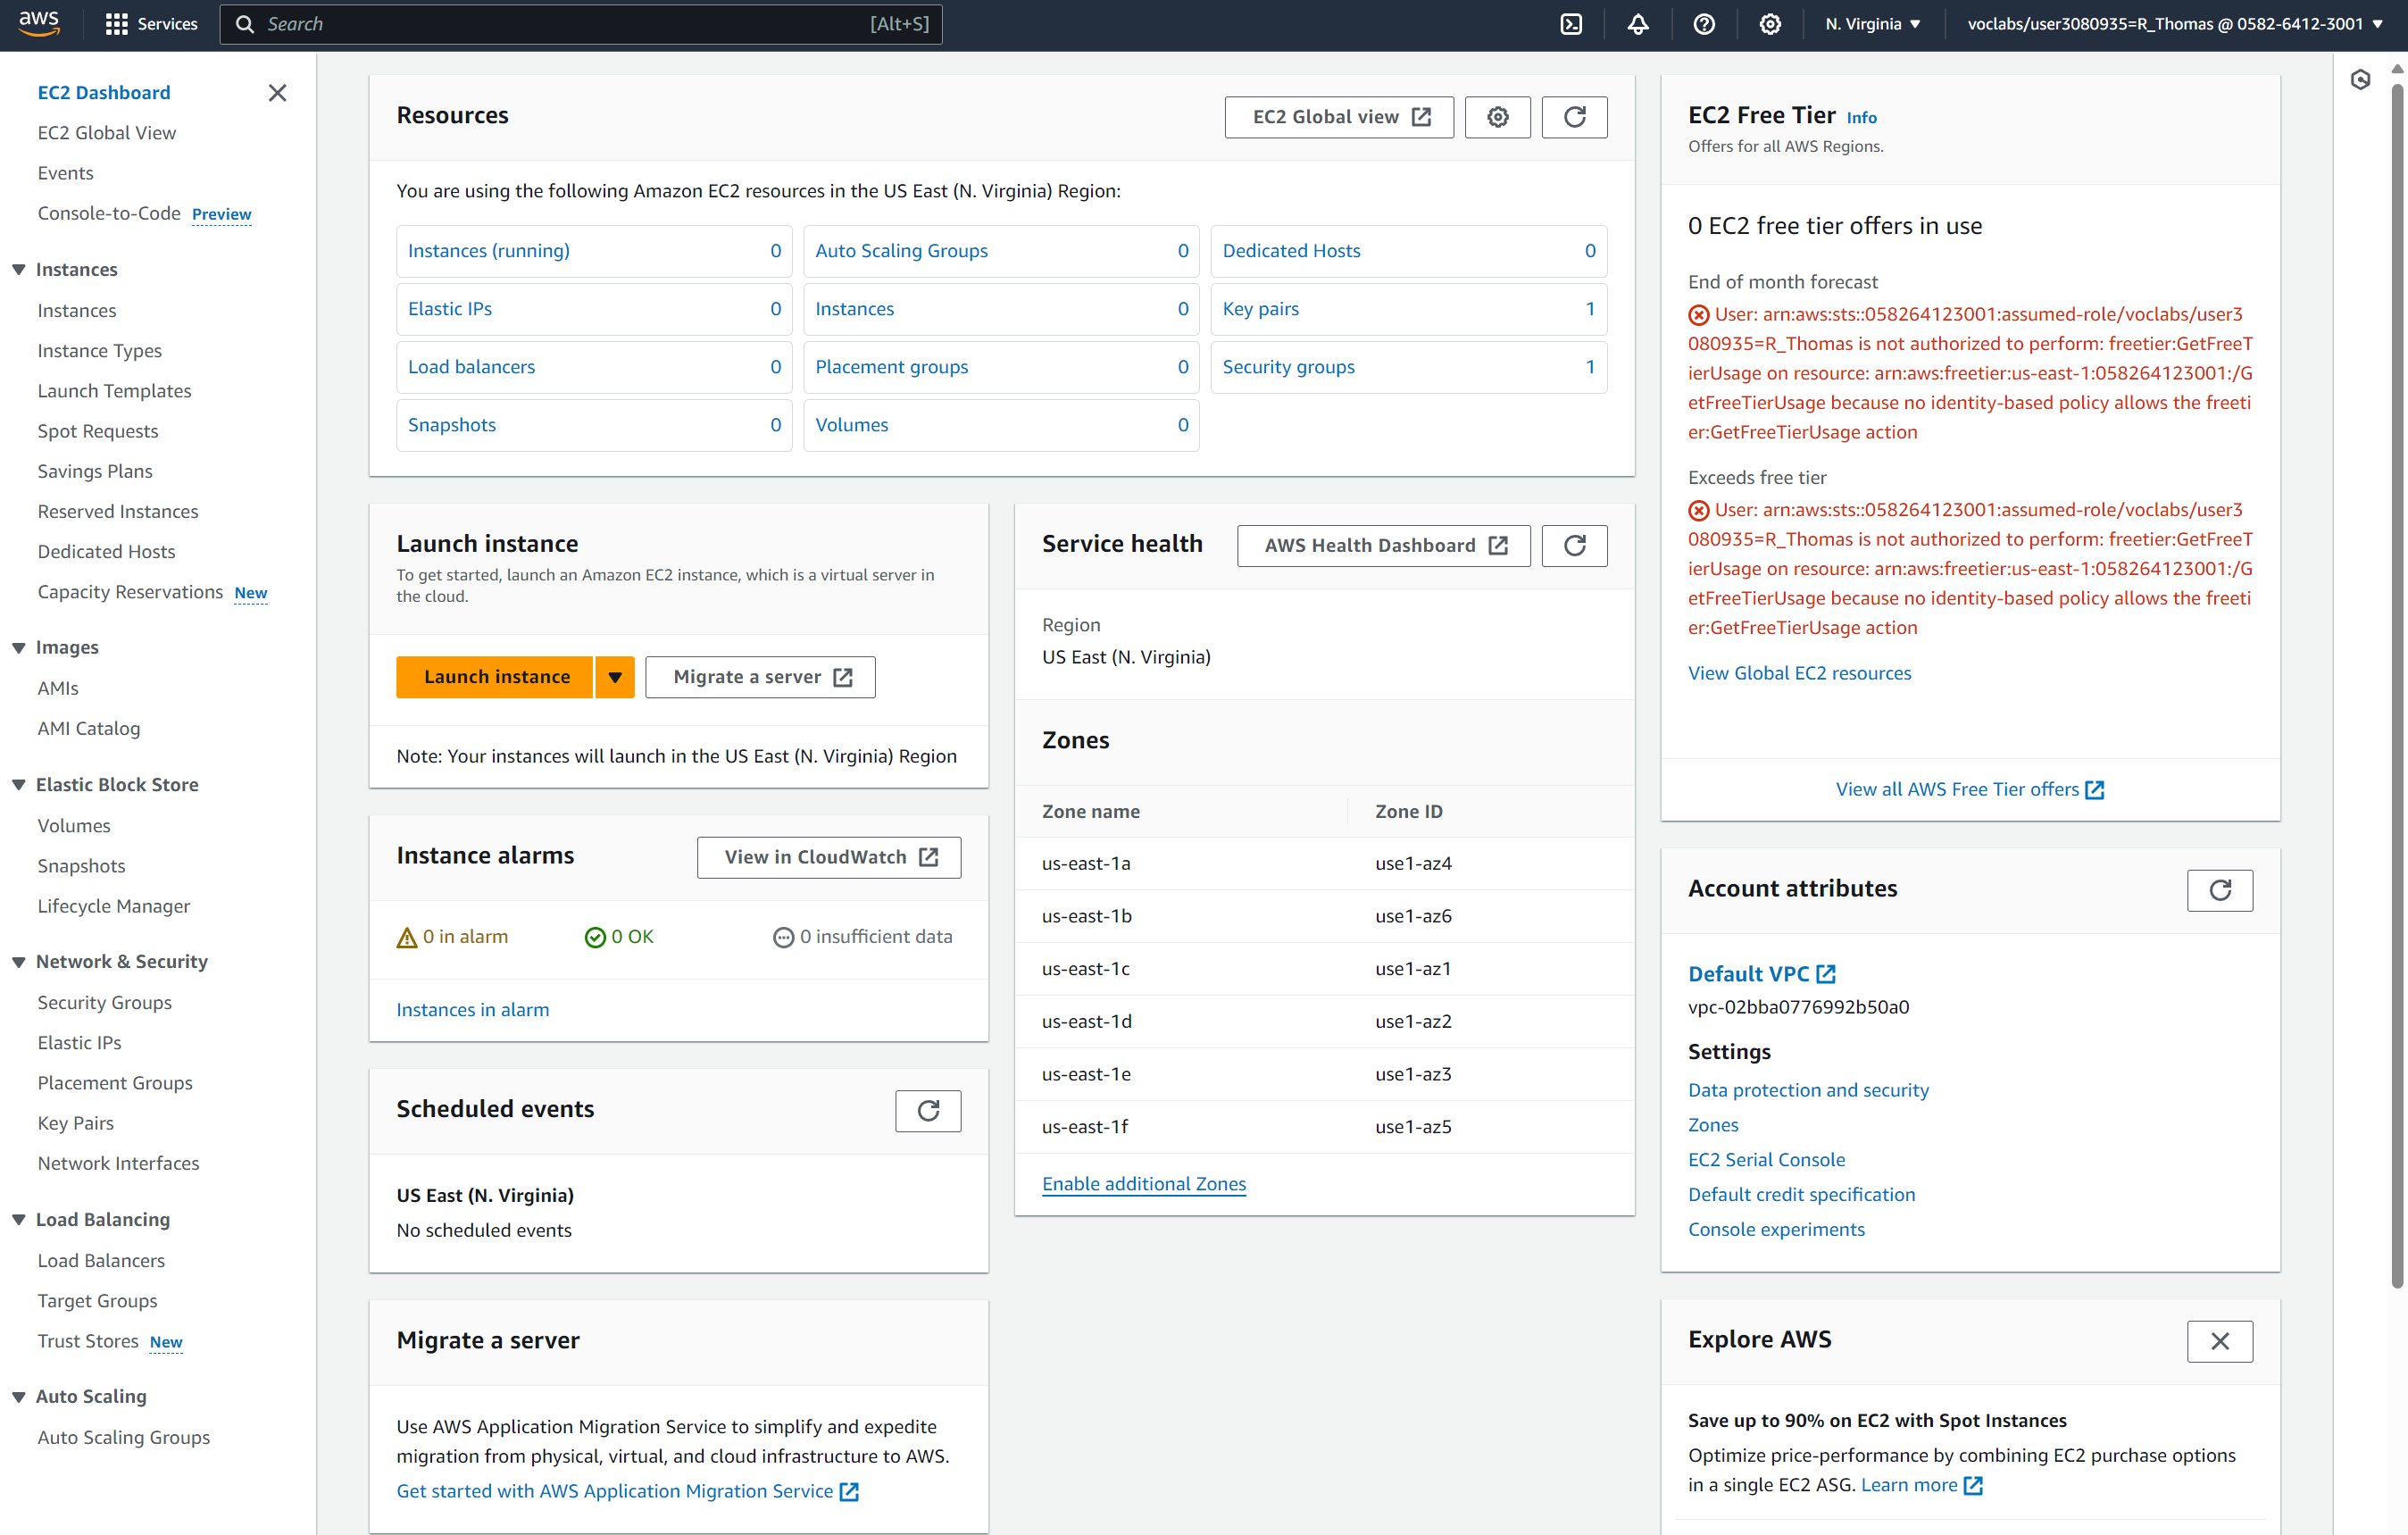
\includegraphics[width=\textwidth]{images/ec2-interface}

\subsection{EC2 AMI}
First we will need to select an Amazon Machine Image (AMI).
An AMI is the template (cookie cutter) which provides instructions on how an instance should be provisioned.
Amazon offers a range of built-in AMIs. There are also community AMIs or you can create your own.
As we just want a simple server today, we will use one of the built-in AMIs.

We will use the Amazon Linux 2023 AMI today,
it is considered one of the fundamental images.
Every AMI has a unique AMI code,
which is \texttt{ami-0e731c8a588258d0d} for the Amazon Linux 2023 AMI.
%Search for it via the code and select it.

\vspace{4mm}
\noindent
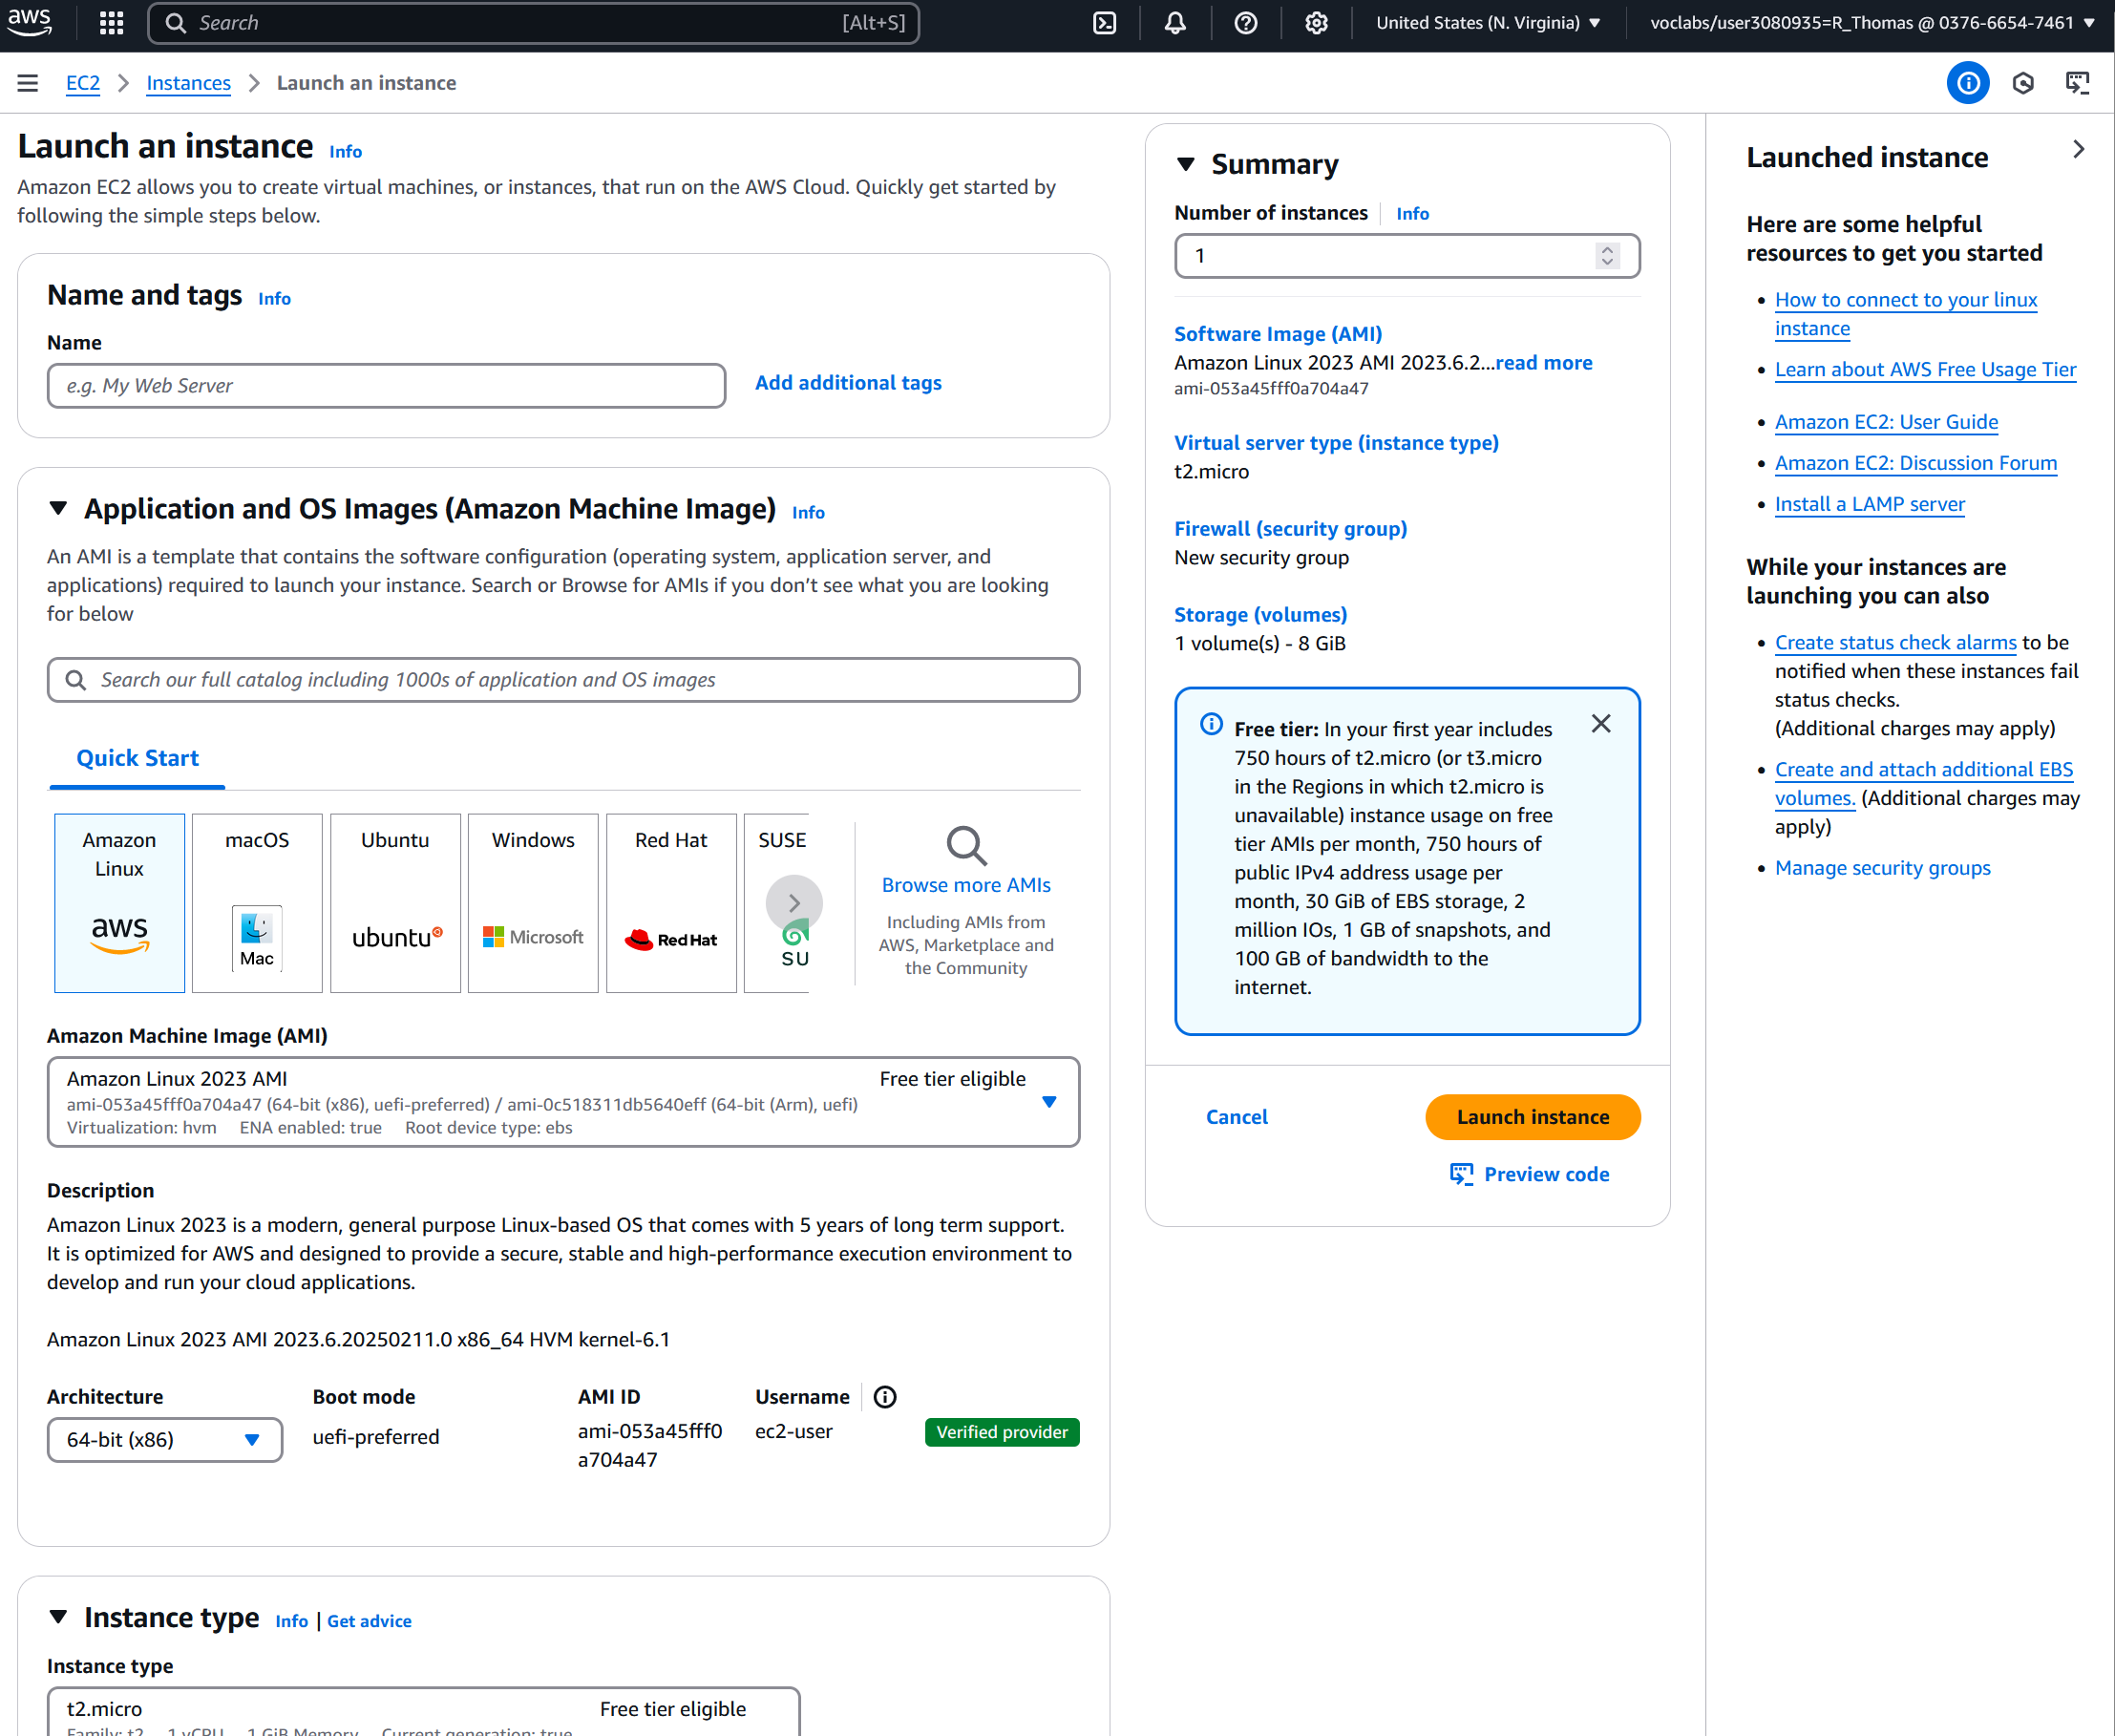
\includegraphics[width=\textwidth]{images/launch-instance}

\teacher{This AMI is a RedHat style distro with yum as its package manager.}

\subsection{Instance Settings}
The settings to configure your instance are:
\begin{enumerate}
\item Add a `Name' tag. Call it the name of your website, e.g. \texttt{hextris}.
\item Select an appropriate AMI, i.e. Amazon Linux 2023 AMI, \texttt{ami-0e731c8a588258d0d}.
\item Select a 64-bit (x86) architecture.
\item The instance type defines the computing, memory, networking and storage capabilities of your instance. We do not need a large server, choose \texttt{t2.micro}.
\item Select the existing \texttt{vockey} (Type: RSA) key pair option.
\item In network settings, choose `Create security group' and select to allow SSH traffic from anywhere, and HTTPS and HTTP access from the internet.
\item Keep the `Configure storage' settings as default.
\item Do not worry about the `Advanced details' options for now.
\item You can now launch the instance to start your server.
\teacher{To make the box pingable dont forget to add the All-ICMP4 with source anywhere.}
\end{enumerate}

\section{Accessing the Instance}

Return to the \texttt{Instances} dashboard.
You should see that a new instance has been created, its instance state might not yet be \texttt{Running}, if not, wait.

\vspace{3mm}
\noindent
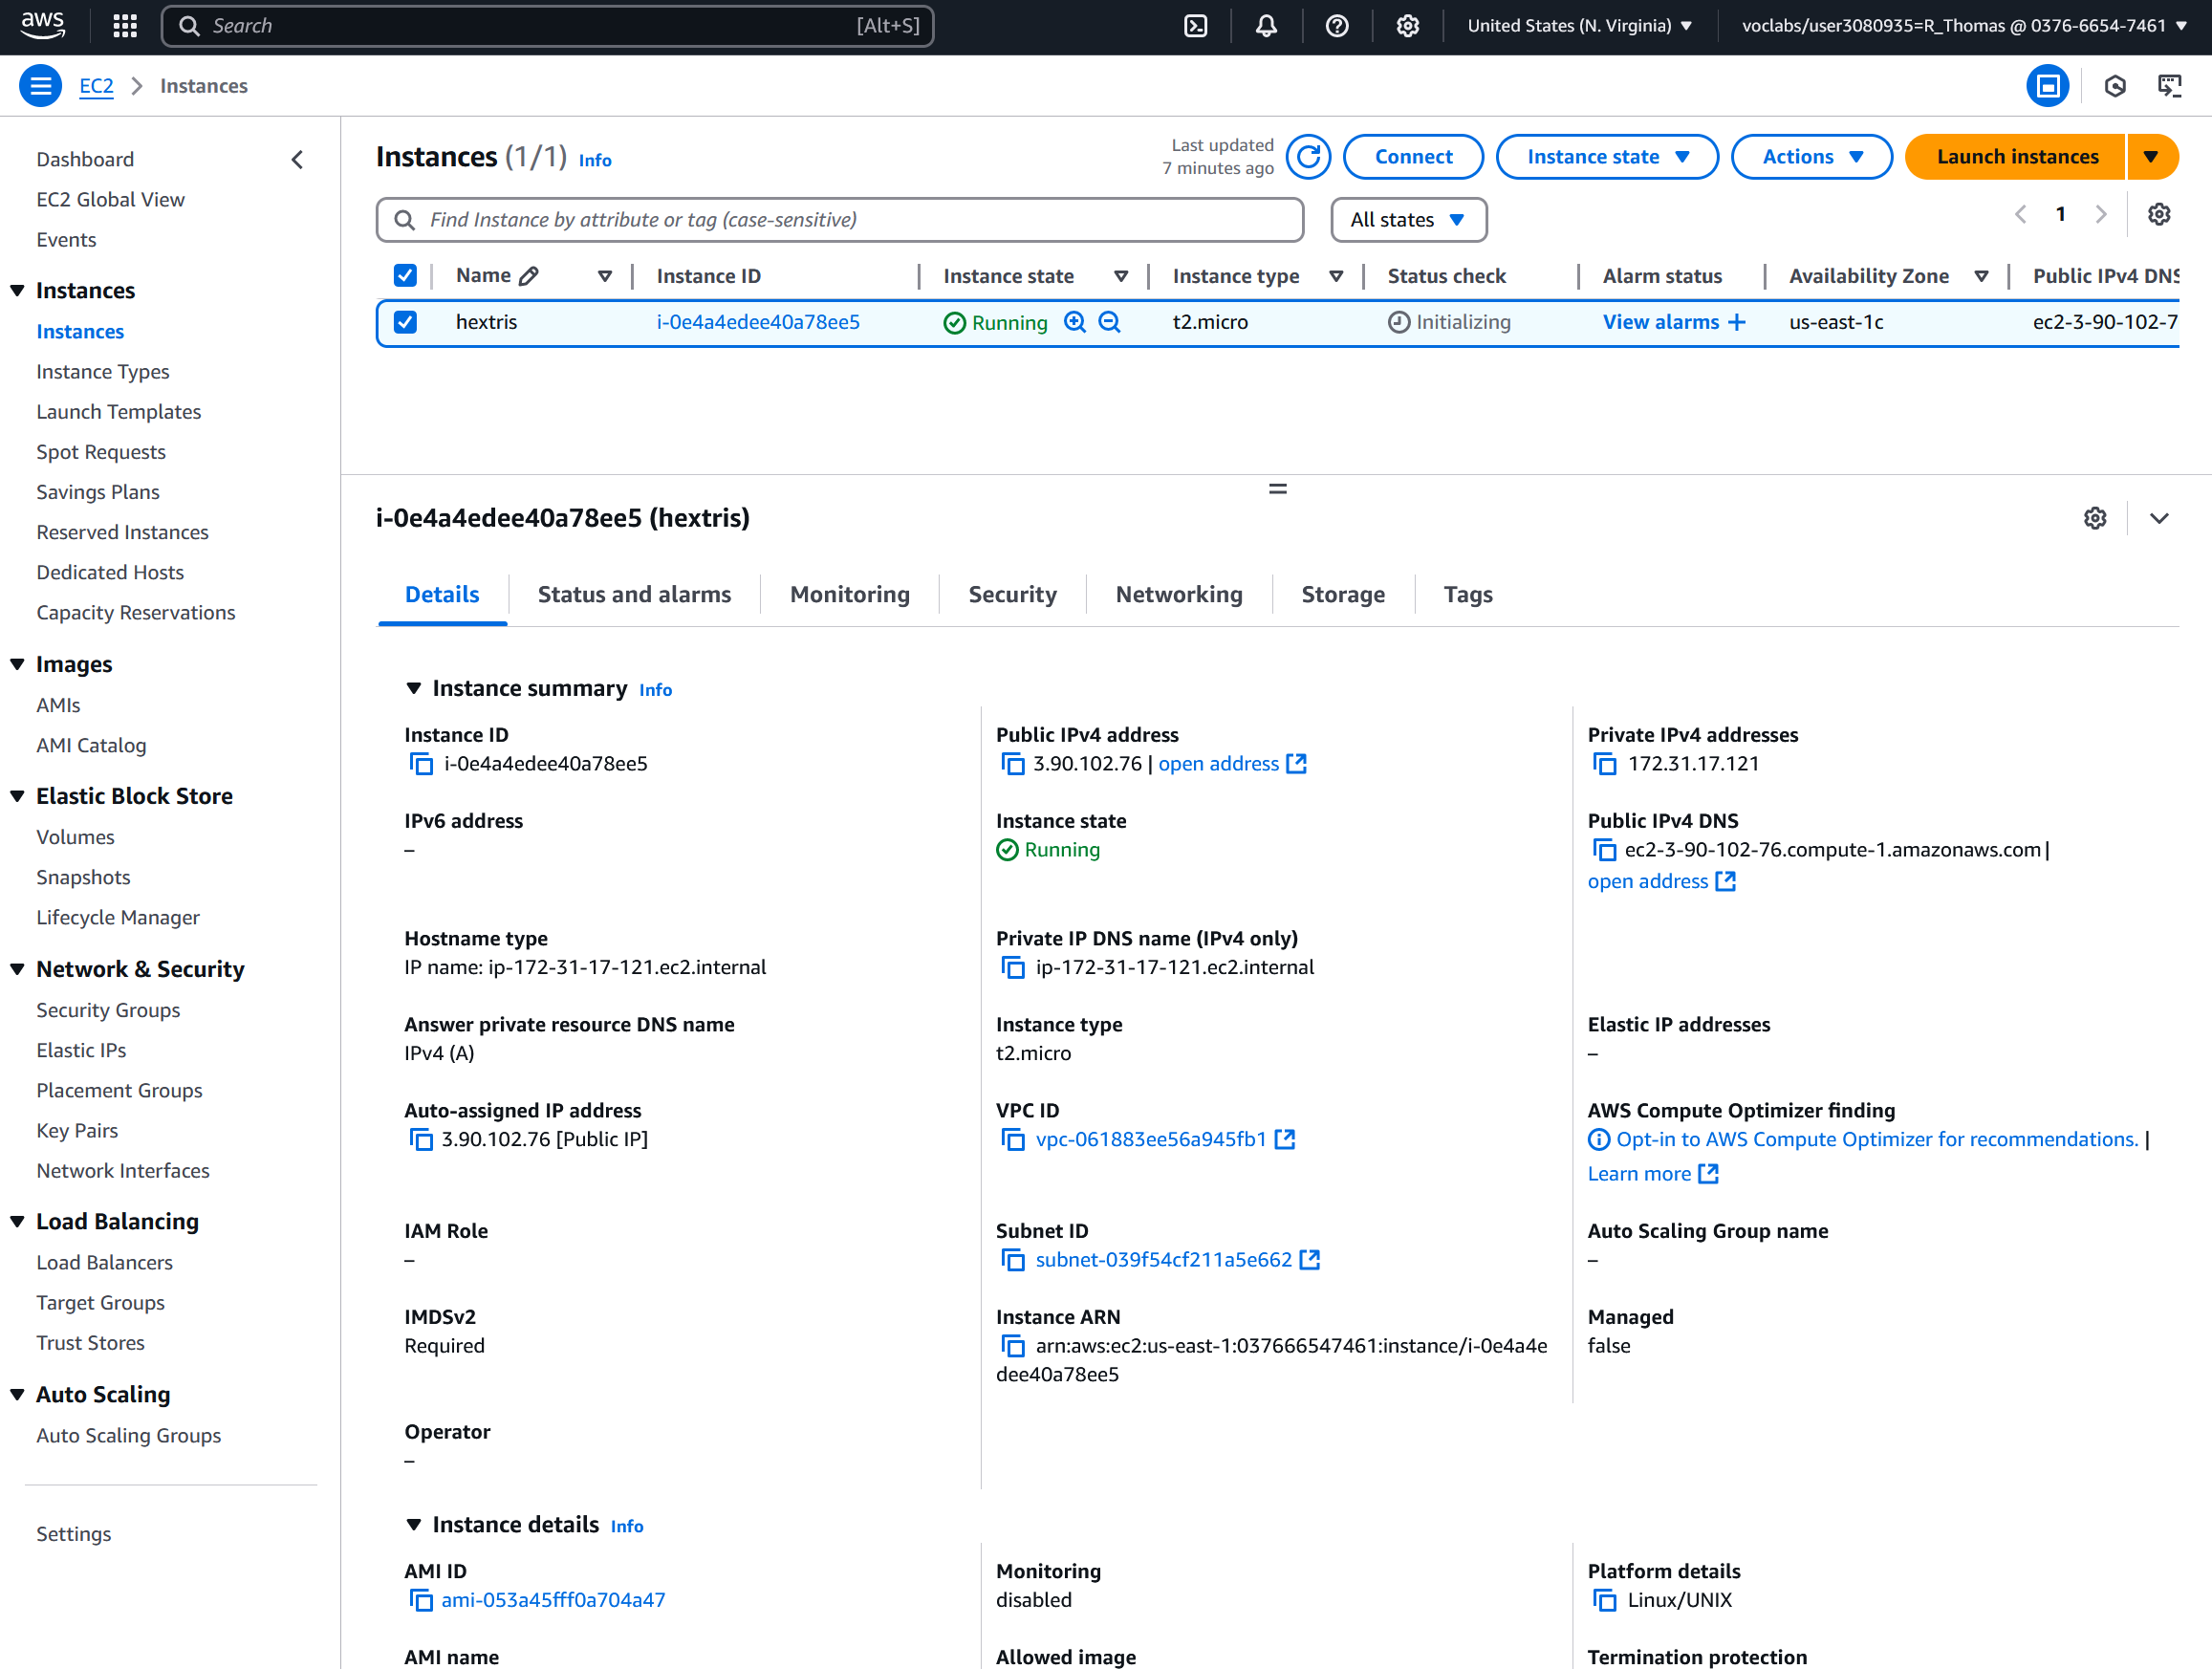
\includegraphics[width=\textwidth]{images/instance-interface}
\vspace{3mm}

\noindent
Note the public IPv4 address as we will need to use this to connect to the server.

\begin{enumerate}
    \item Return to the AWS Learner Lab interface.
    \item Run the following, \textcolor{red}{replacing \texttt{127.0.0.1}} with the public IP address of your instance.
          This command uses the \texttt{vockey | RSA} key pair to gain SSH access to the machine.
\end{enumerate}
\bash{ssh -i ~/.ssh/labsuser.pem ec2-user@127.0.0.1}

For example:
\hspace{5mm}
\vtop{
  \vskip0pt
  \hbox{
    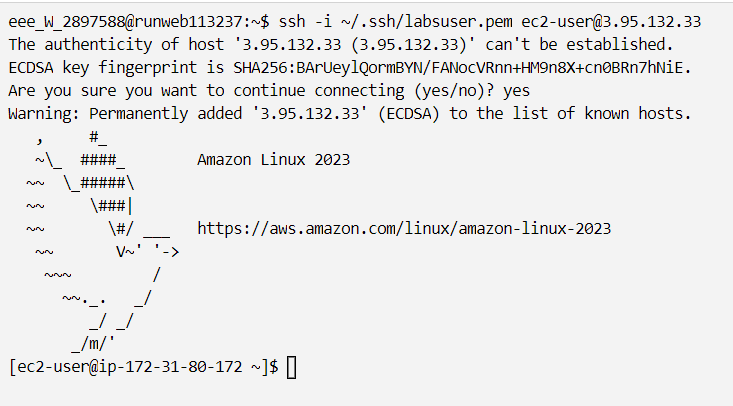
\includegraphics{images/access-instance}
  }
}

% Can't get ASCII art to display correctly when processed.
%
%\begin{code}[language=bash,numbers=none]{}
%ddd_v1_644362@runweb75312:~$ ssh -i ~/.ssh/labsuser.pem ec2-user@35.173.230.42
%The authenticity of host '35.173.230.42 (35.173.230.42)' can't be established.
%ECDSA key fingerprint is SHA256:W7OzzZm6nhwM9tB9Kb7enONPryo1a4259hJmSAZX7HQ.
%Are you sure you want to continue connecting (yes/no)? yes
%
%# At this point you will want to type yes and press enter
%Warning: Permanently added '35.173.230.42' (ECDSA) to the list of known hosts.
%   ,     #_
%   ~\_  ####_        Amazon Linux 2023
%  ~~  \_#####\
%  ~~     \###|
%  ~~       \#/ ___   https://aws.amazon.com/linux/amazon-linux-2023
%   ~~       V~' '->
%    ~~~         /
%      ~~._.   _/
%         _/ _/
%       _/m/'
%
%https://aws.amazon.com/amazon-linux-2/
%[ec2-user@ip-172-31-53-4 ~]$
%\end{code}

\section{Installing Hextris}\label{sec:installHextris}
Hextris \cite{hextris} is very simple to install, using an EC2 interface is perhaps overkill for it.
It is an entirely client-side/static web application which means we just have to serve the static files.

First, we will need to enable serving of static files.
We can install and start the \texttt{httpd} service for this.
The AMI we have picked uses the yum package manager, so to install httpd we run:

\begin{code}[language=bash,numbers=none]{}
> sudo yum install httpd
Last metadata expiration check: ...
Dependencies resolved
..... 
..... 
Total download size: 2.3 M
Installed size: 6.9 M
Is this ok [y/N]:

# enter y to install
..... 
..... 
Complete!
> sudo systemctl enable httpd
Created symlink from /etc/systemd/system/multi-user.target.wants/httpd.service to /usr/lib/systemd/system/httpd.service.
> sudo systemctl start httpd
\end{code}

All files in the \texttt{/var/www/html} directory will now be served when accessed via HTTP.
Navigate to the public IP address of your EC2 instance in the browser.
You should see an ``It works!'' landing page.

Change to the \texttt{/var/www/html} directory and notice that it is currently empty.
We need to download the static files to this directory so that they can be served.
We can use git for this (though it is not the most suited tool),
but first git needs to be installed on the instance.

\bash{sudo yum install git}

Finally, confirm that we are in the \texttt{/var/www/html} directory.

\bash{cd /var/www/html}

\teacher{This path will currently be owned by root, proper permissions can be done (but are not nesscary) by following \url{https://docs.aws.amazon.com/AmazonRDS/latest/UserGuide/CHAP_Tutorials.WebServerDB.CreateWebServer.html}}

And clone the repository into that directory.

\bash{sudo git clone https://github.com/Hextris/hextris .}

\teacher{Mention to not forget about the "." as it is easily missed.}
\teacher{If git is prompting for a username and password then there may be a typo in the repository url.}

Now if you navigate to the \textbf{http} address of the public IP address (e.g. \url{http://18.208.165.253}), you should be able to see your newly deployed website.
Congratulations!

\notice{If you are having timeout issues,
one problem could be using \texttt{https} to connect rather than \texttt{http}.}

\teacher{Make sure they delete their instances.}

\section{Switching to Terraform}

For the remainder of the practical we will be using Terraform to provision the same instance we just created.

\begin{enumerate}
    \item First, please delete any running instances in your AWS account using the AWS Console.
    \item Next, navigate to the GitHub Classroom link for this practical provided by your tutor.
    This will create a new repository where we can work on Terraform.
\end{enumerate}

\section{Using Terraform in AWS Learner Labs}
We will redeploy our Hextris application using Infrastructure as Code (IaC) to do so.
You will need to keep your lab running for the next steps.
(Now is a good time to click start to refresh your 4 hours.)

\begin{enumerate}
\item Click on `AWS Details' to display information about the lab.

\hspace{-4mm}
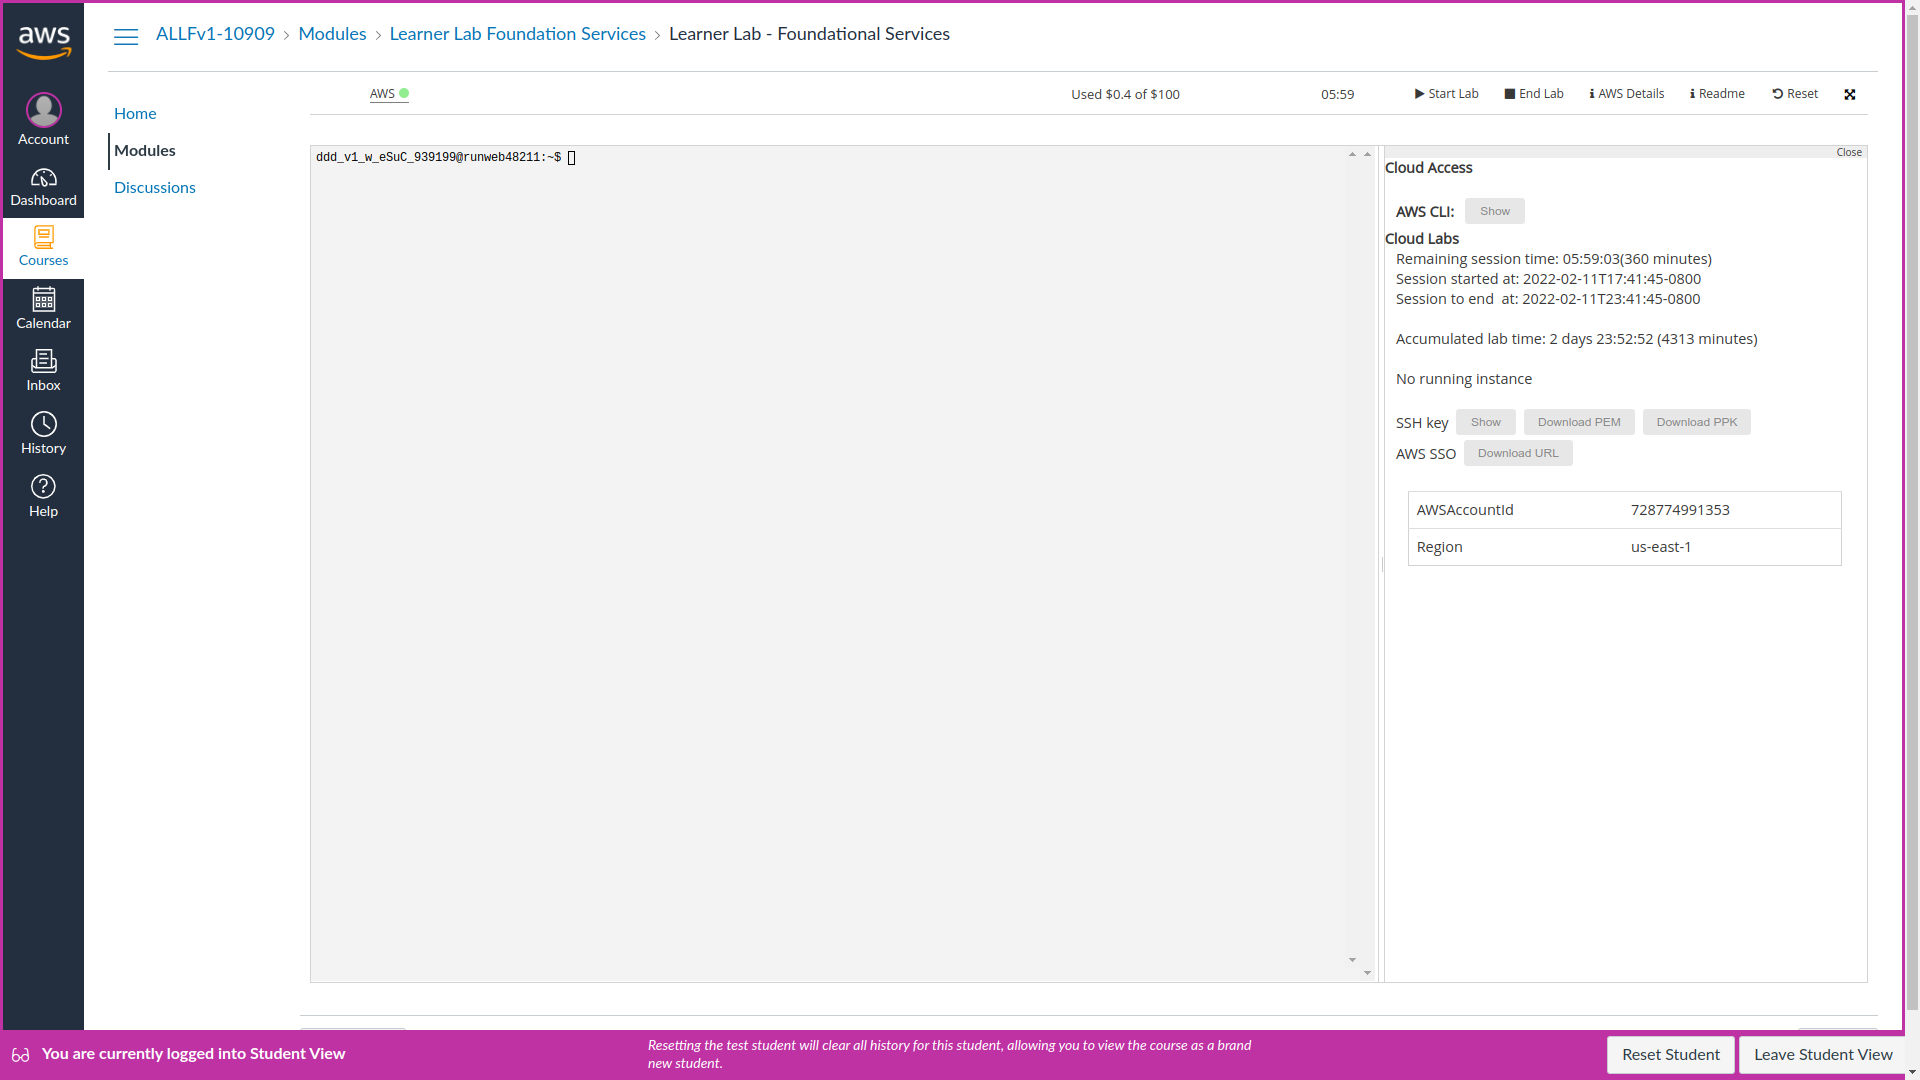
\includegraphics[width=\textwidth]{images/aws-details}

\item Click on the first `Show' button next to `AWS CLI' which will display a text block starting with \texttt{[default]}.
\item Within your repository create a \texttt{credentials} file and copy the contents of the text block into the file.
\textbf{Do not share this file contents --- do not commit it}.
This file is added to the \texttt{.gitignore} of your repository by default.
\item Create a \texttt{main.tf} file in the same directory with the following contents:
\begin{code}[language=terraform,numbers=none]{main.tf}
terraform {
    required_providers {
        aws = {
            source  = "hashicorp/aws"
            version = "~> 5.0"
        }
    }
}

provider "aws" {
    region = "us-east-1"
    shared_credentials_files = ["./credentials"]
}
\end{code}

The \texttt{terraform} block specifies the required external dependencies, here we need to use the AWS provider above version 5.0.
The \texttt{provider} block configures the AWS provider, instructing it which region to use and how to authenticate (using the credentials file we created).

\item We need to initialise Terraform which will download the required dependencies.
    This is done with the \texttt{terraform init} command.
\bash{terraform init}

This command will create a \texttt{.terraform} directory which stores providers and a provider lock file, \texttt{.terraform.lock.hcl}.

\item To verify that we have setup Terraform correctly, use \texttt{terraform plan}.
\bash{terraform plan}

As we currently have no resources configured, it should find that no changes are required.
Note that this does not ensure our credentials are correctly configured, as Terraform has no reason to try authenticating yet.

\end{enumerate}

\section{Deploying Hextris}
First, we will need to create an EC2 instance resource.
The AWS provider calls this resource an \link{\texttt{aws\_instance}}{https://registry.terraform.io/providers/hashicorp/aws/latest/docs/resources/instance}.
Get familiar with the documentation page.
Most Terraform providers have reasonable documentation.
Reading the argument reference section helps to understand what a resource is capable of.

We will start off with the basic information for the resource.
Configure it to use a specific Amazon Machine Instance (AMI) and chose the \texttt{t2.micro} size.
We will also give it a name so that it is easy to find.
Add the following basic resource to \texttt{main.tf}:

\begin{code}[language=terraform,numbers=none]{main.tf}
resource "aws_instance" "hextris-server" {
    ami           = "ami-005f9685cb30f234b"
    instance_type = "t2.micro"
    key_name      = "vockey"
    
    tags = {
        Name = "hextris"
    }
}      
\end{code}

To create the server, invoke
\texttt{terraform apply} which will first do \texttt{terraform plan} and prompt us to confirm if we want to apply changes.

\bash{terraform apply}

You should be prompted with something similar to the output below.

\begin{code}[numbers=none]{}
Terraform used the selected providers to generate the following execution plan. Resource actions are indicated with the following symbols:
  + create

Terraform will perform the following actions:

  # aws_instance.hextris-server will be created
  + resource "aws_instance" "hextris-server" {
      + ami                                  = "ami-005f9685cb30f234b"
      (omitted)
      + instance_type                        = "t2.micro"
      (omitted)
      + tags                                 = {
          + "Name" = "hextris"
        }
    }

Plan: 1 to add, 0 to change, 0 to destroy.

Do you want to perform these actions?
  Terraform will perform the actions described above.
  Only 'yes' will be accepted to approve.

  Enter a value: 
\end{code}

If the plan looks sensible enter \texttt{yes} to enact the changes.

\begin{code}[numbers=none]{}
  Enter a value: yes

aws_instance.hextris-server: Creating...
aws_instance.hextris-server: Still creating... [10s elapsed]
aws_instance.hextris-server: Still creating... [20s elapsed]
aws_instance.hextris-server: Still creating... [30s elapsed]
aws_instance.hextris-server: Still creating... [40s elapsed]
aws_instance.hextris-server: Creation complete after 47s [id=i-08c92a097ae7c5b18]

Apply complete! Resources: 1 added, 0 changed, 0 destroyed.
\end{code}

You can now check in the AWS Console that another EC2 instance with the name \texttt{hextris} has been created.
Now that we have a server, we should try to configure it to serve Hextris.
We will use the \texttt{user\_data} field which configures commands to run when launching the instance.
First we need a script to provision the server, if we combine all our commands from section \ref{sec:installHextris}, we will produce this script:

\begin{code}[language=bash,numbers=none]{serve-hextris.sh}
#!/bin/bash
yum install -y httpd
systemctl enable httpd
systemctl start httpd

yum install -y git
cd /var/www/html
git clone https://github.com/Hextris/hextris .  
\end{code}

\teacher{The hash bang is required.}

\teacher{Don't forget the -y on yum install}

Now we can add the following field to our Terraform resource.
It uses the Terraform \texttt{file} function to load the contents of a file named \texttt{serve-hextris.sh} relative to the Terraform directory.
The contents of that file is passed to the \texttt{user\_data} field.

\begin{code}[language=terraform,numbers=none]{}
user_data = file("./serve-hextris.sh")
\end{code}

If you run the \texttt{terraform plan} command now,
you will notice that Terraform has identified that this change will require creating a new EC2 instance.
Where possible, Terraform will try to update a resource in-place but since this changes how an instance is started, it needs to be replaced.
Go ahead and apply the changes.

Now, in theory, we should have deployed Hextris to an EC2 instance.
But how do we access that instance?
We \textsl{could} go to the AWS Console and find the public IP address.
However, it turns out that Terraform already knows the public IP address.
In fact, if you open the Terraform state file (\texttt{terraform.tfstate}),
you should be able to find it hidden away in there.
But we do not want to go hunting through this file all the time.
Instead we will use the \texttt{output} keyword.

We can specify certain attributes as `output' attributes.
Output attributes are printed to the terminal when the module is invoked directly
but as we will see later, they can also be used by other Terraform configuration files.

\begin{code}[language=terraform,numbers=none]{main.tf}
output "hextris-url" {
  value = aws_instance.hextris-server.public_ip
}
\end{code}

This creates a new output attribute, \texttt{hextris-url},
which references the \texttt{public\_ip} attribute of our \texttt{hextris-server} resource.
Note that resources in Terraform are addressed by the resource type (\texttt{aws\_instance})
followed by the name of the resource (\texttt{hextris-server}).

If you plan or apply the changes, it should tell you the public IP address of the instance resource.
\bash{terraform plan}

\begin{code}[numbers=none]{}
aws_instance.hextris-server: Refreshing state... [id=i-043a61ff86aa272e0]

Changes to Outputs:
  + hextris-url = "3.82.225.65"
\end{code}

You can apply this plan to save these new output values to the Terraform state, without changing any real infrastructure.  

So let's try and access that URL, hmm.
That is strange. Something has gone wrong.

\section{Security Groups}
When we setup our EC2 instance using the AWS Console,
it helpfully created a new security group for us.
We specified that this security group should allow SSH, HTTP, and HTTPS traffic by allowing traffic from ports 22, 80, and 443 respectively.
When configuring with Terraform, security groups and their attachment to EC2 instances are separate resources.
Refer back to the Terraform documentation for details or,
as is normally quicker, \href{https://www.google.com/search?q=terraform+aws+security+group}{Google ``terraform aws security group''}.

First, let us create an appropriate security group.
Recall that in the AWS Console configuration,
ingress SSH access (port 22) and all egress%
\footnote{Ingress and egress in networking just means incoming and outgoing respectively.}
traffic was automatically configured and we just added ingress port 80.
In Terraform the whole state must be configured so we specify two
\texttt{ingress} blocks one for HTTP (port 80) and one for SSH access (port 22).%
\footnote{We do not actually need SSH access as all the server configuration is done when the machine is provisioned thanks to the \texttt{user\_data},
but we are trying to create a new instance that is identical to the original AWS Console in section \ref{sec:installHextris}.}
Additionally, we will create egress for all outgoing traffic.

\begin{code}[language=terraform,numbers=none]{}
resource "aws_security_group" "hextris-server" {
  name = "hextris-server"
  description = "Hextris HTTP and SSH access"

  ingress {
    from_port = 80
    to_port = 80
    protocol = "tcp"
    cidr_blocks = ["0.0.0.0/0"]
  }

  ingress {
    from_port = 22
    to_port = 22
    protocol = "tcp"
    cidr_blocks = ["0.0.0.0/0"]
  }

  egress {
    from_port = 0
    to_port = 0
    protocol = "-1"
    cidr_blocks = ["0.0.0.0/0"]
  }
}
\end{code}

Note the following:
\begin{itemize}
  \item \texttt{from\_port} and \texttt{to\_port} are the start and end of a range of ports rather than incoming or outgoing. In this example our range is 80-80.
  \item \texttt{protocol} set to -1 is a special flag to indicate all protocols.
  \item Explaining \texttt{cidr} is outside the scope of the course, but the specified block above means to apply to all IP addresses.
\end{itemize}

You may now apply the changes to create this new security group resource.

Next, we will attach the security group to the EC2 instance.
Return to the \texttt{aws\_instance.hextrix-server} resource
and include the following line:

\begin{code}[language=terraform,numbers=none]{}
security_groups = [aws_security_group.hextris-server.name]
\end{code}

Note that EC2 instances can have multiple security groups.
Once again notice the structure of resource identifiers in AWS.

% Now if we try to apply or plan these changes,
% we'll noticed that the change of security group forces replacement.
% TODO: I don't actually know why it does this.

Now apply the changes.
If you now try to access via the IP address
(the IP address may have changed),
you should be able to view the hextris website.

\section{Tearing Down}

One of the important features of Infrastructure as Code (IaC) is all the configuration we just did is stored in a file.
This file can, and should be, version controlled and subject to the same quality rules of code files.
It also means that if we want to redeploy Hextris at any point,
we can easily just run the IaC to deploy it.

To try this out, let us first take everything down.
We can do this with:
\bash{terraform destroy}

You should be prompted to confirm that you want to destroy all of the resources in the state.
Once Terraform has finished taking everything down,
confirm that you can no longer access the website and that the AWS console says the instances have been destroyed.

Now go ahead and apply the changes to bring everything back:
\bash{terraform apply}

Confirm that this brings the website back exactly as before (with a different IP address).
You can now start any lab you want and almost instantly spin back up the website you have configured.
That is the beauty of Infrastructure as Code!

\textbf{Hint:} Destroy everything again before you finish.

\section{Automated Testing}
A quick note about automated testing.
As with all the practicals thus far,
this practical has automated tests enabled on your repository.

From within your repository, you can run the tests locally with:
\bash{.csse6400/bin/unittest.sh}

While the emails saying that the tests failed can be annoying,
these automated tests allow us to ensure that everyone is keeping up with the practical content.

If fixing the test failures is not too hard,
please try to do so.
If you are repeatedly not passing the practicals,
we may reach out to ensure that you are not being left behind in the content.


\bibliographystyle{ieeetr}
\bibliography{regions,hextris,ours,books}

\appendix

% \teacher{
\section{AWS Networking Terminology}
\paragraph{AWS Regions}
Regions are the physical locations of AWS data centres.
When applying Terraform, the changes are being made to one region at a time.
In our case we specified the region \texttt{us-east-1}.
Often you do not need to deploy to more than one region, however,
it can help decrease latency and reduce risk from a major disaster.
Generally, pick a region and stick with it,
we have picked \texttt{us-east-1} because it is the least expensive.

\begin{figure}[ht]
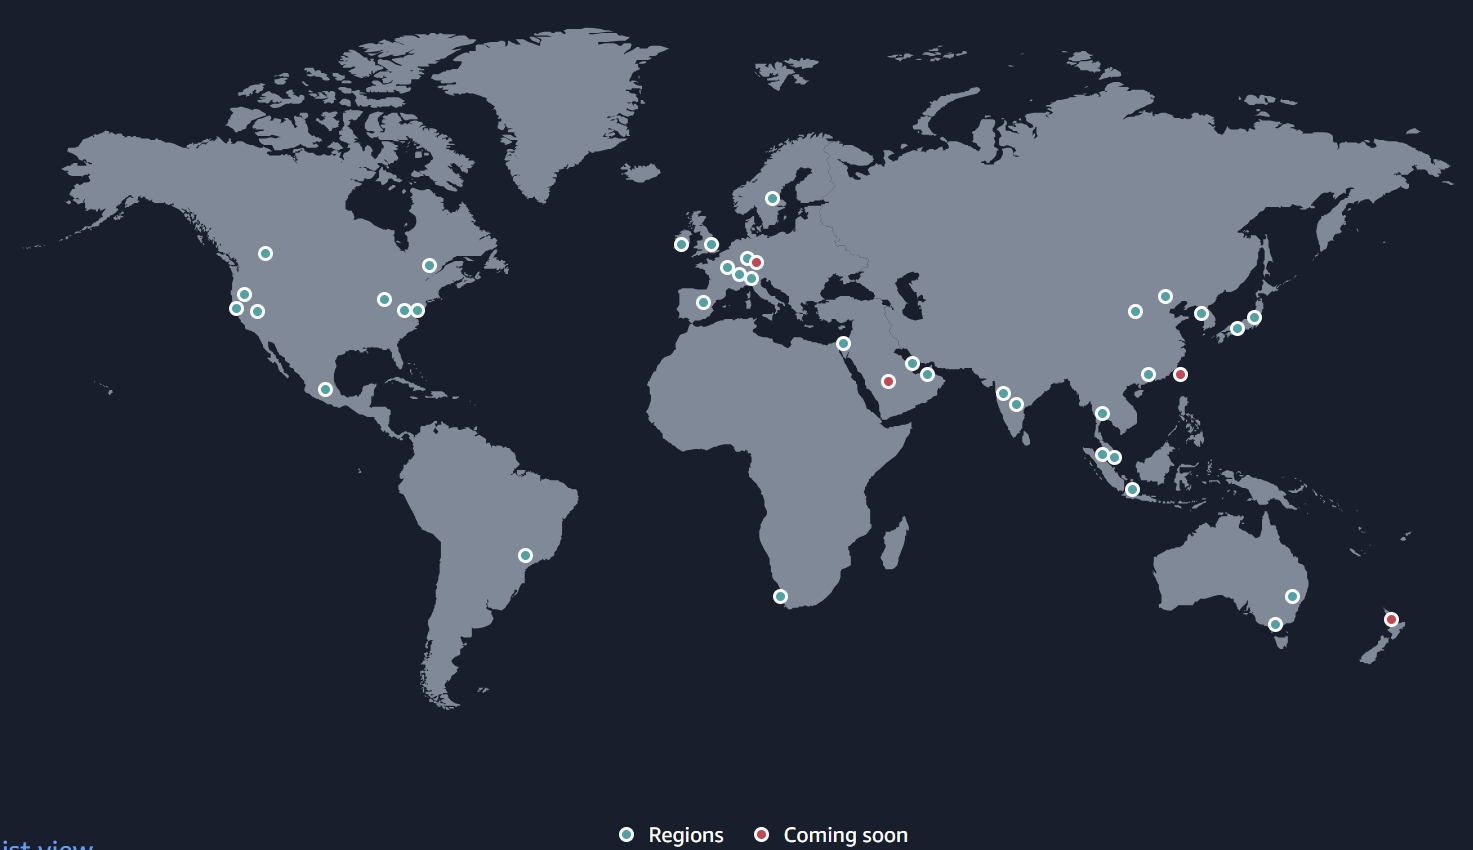
\includegraphics[width=\textwidth]{images/aws_regions}
\caption{AWS Regions as of February 2024 \cite{aws-regions}}
\end{figure}

\paragraph{Availability Zones}
An AWS Region will consist of availability zones, normally named with letters.
For example, the AWS Region located in Sydney, \texttt{ap-southeast-2} has three availability zones:
\texttt{ap-southeast-2a}, \texttt{ap-southeast-2b}, and \texttt{ap-southeast-2c}.
An availability zone is a collection of resources which run on separate power supplies and networks.
Essentially minimising the risk that multiple availability zones would fail at once.

\paragraph{VPC}
Virtual Private Clouds, or VPCs,
are virtual networks under your control,
if you have managed a regular network before it should be familiar.
VPCs are contained within one region but are spread across multiple availability zones.


\end{document}
